\documentclass{article}
\usepackage[final]{neurips_2025}  % NEURIPS style (neurips_2025.sty is in paper_draft/)
% neurips_2025.sty leaves \@trackname undefined when only [final] is passed (no track option).
% Left empty so the footer does not claim a venue; add the `main' option to restore the notice.
\makeatletter\providecommand{\@trackname}{}\makeatother
\usepackage[hidelinks]{hyperref}  % REQUIRED: clickable links
\usepackage{booktabs}  % REQUIRED: professional tables
\usepackage{graphicx}
\usepackage{amsmath,amssymb}
\usepackage[utf8]{inputenc}
\usepackage[T1]{fontenc}
\usepackage{enumitem}
\usepackage{multirow}
\usepackage{caption}
\usepackage{algorithm}
\usepackage[noend]{algpseudocode}

% Import command files
%%%%% MATH NOTATION MACROS %%%%%
% Standard math notation for academic papers
% Import with: %%%%% MATH NOTATION MACROS %%%%%
% Standard math notation for academic papers
% Import with: %%%%% MATH NOTATION MACROS %%%%%
% Standard math notation for academic papers
% Import with: \input{commands/math}

\usepackage{amsmath,amsfonts,bm}

%%%%%%%%%%%%%%%%%%%%%%%%%%%%%%%%%%%%%%%%%%%%%%%%%%%%%%%%%%%%%%%%%
% FIGURE AND SECTION REFERENCES
%%%%%%%%%%%%%%%%%%%%%%%%%%%%%%%%%%%%%%%%%%%%%%%%%%%%%%%%%%%%%%%%%

% Mark sections of captions for referring to divisions of figures
\newcommand{\figleft}{{\em (Left)}}
\newcommand{\figcenter}{{\em (Center)}}
\newcommand{\figright}{{\em (Right)}}
\newcommand{\figtop}{{\em (Top)}}
\newcommand{\figbottom}{{\em (Bottom)}}
\newcommand{\captiona}{{\em (a)}}
\newcommand{\captionb}{{\em (b)}}
\newcommand{\captionc}{{\em (c)}}
\newcommand{\captiond}{{\em (d)}}

% Figure references
\def\figref#1{figure~\ref{#1}}
\def\Figref#1{Figure~\ref{#1}}
\def\twofigref#1#2{figures \ref{#1} and \ref{#2}}
\def\quadfigref#1#2#3#4{figures \ref{#1}, \ref{#2}, \ref{#3} and \ref{#4}}

% Section references
\def\secref#1{section~\ref{#1}}
\def\Secref#1{Section~\ref{#1}}
\def\twosecrefs#1#2{sections \ref{#1} and \ref{#2}}
\def\secrefs#1#2#3{sections \ref{#1}, \ref{#2} and \ref{#3}}

% Equation references
\def\eqref#1{equation~\ref{#1}}
\def\Eqref#1{Equation~\ref{#1}}
\def\plaineqref#1{\ref{#1}}

% Algorithm references
\def\algref#1{algorithm~\ref{#1}}
\def\Algref#1{Algorithm~\ref{#1}}
\def\twoalgref#1#2{algorithms \ref{#1} and \ref{#2}}
\def\Twoalgref#1#2{Algorithms \ref{#1} and \ref{#2}}

% Table references
\def\tabref#1{table~\ref{#1}}
\def\Tabref#1{Table~\ref{#1}}

% Chapter references
\def\chapref#1{chapter~\ref{#1}}
\def\Chapref#1{Chapter~\ref{#1}}

%%%%%%%%%%%%%%%%%%%%%%%%%%%%%%%%%%%%%%%%%%%%%%%%%%%%%%%%%%%%%%%%%
% BASIC MATH DEFINITIONS
%%%%%%%%%%%%%%%%%%%%%%%%%%%%%%%%%%%%%%%%%%%%%%%%%%%%%%%%%%%%%%%%%

\def\ceil#1{\lceil #1 \rceil}
\def\floor#1{\lfloor #1 \rfloor}
\def\1{\bm{1}}
\def\eps{{\epsilon}}

% Common operators
\DeclareMathOperator*{\argmax}{arg\,max}
\DeclareMathOperator*{\argmin}{arg\,min}
\DeclareMathOperator{\sign}{sign}
\DeclareMathOperator{\Tr}{Tr}
\let\ab\allowbreak

%%%%%%%%%%%%%%%%%%%%%%%%%%%%%%%%%%%%%%%%%%%%%%%%%%%%%%%%%%%%%%%%%
% VECTORS (lowercase bold)
%%%%%%%%%%%%%%%%%%%%%%%%%%%%%%%%%%%%%%%%%%%%%%%%%%%%%%%%%%%%%%%%%

\def\vzero{{\bm{0}}}
\def\vone{{\bm{1}}}
\def\vmu{{\bm{\mu}}}
\def\vtheta{{\bm{\theta}}}
\def\va{{\bm{a}}}
\def\vb{{\bm{b}}}
\def\vc{{\bm{c}}}
\def\vd{{\bm{d}}}
\def\ve{{\bm{e}}}
\def\vf{{\bm{f}}}
\def\vg{{\bm{g}}}
\def\vh{{\bm{h}}}
\def\vi{{\bm{i}}}
\def\vj{{\bm{j}}}
\def\vk{{\bm{k}}}
\def\vl{{\bm{l}}}
\def\vm{{\bm{m}}}
\def\vn{{\bm{n}}}
\def\vo{{\bm{o}}}
\def\vp{{\bm{p}}}
\def\vq{{\bm{q}}}
\def\vr{{\bm{r}}}
\def\vs{{\bm{s}}}
\def\vt{{\bm{t}}}
\def\vu{{\bm{u}}}
\def\vv{{\bm{v}}}
\def\vw{{\bm{w}}}
\def\vx{{\bm{x}}}
\def\vy{{\bm{y}}}
\def\vz{{\bm{z}}}

%%%%%%%%%%%%%%%%%%%%%%%%%%%%%%%%%%%%%%%%%%%%%%%%%%%%%%%%%%%%%%%%%
% MATRICES (uppercase bold)
%%%%%%%%%%%%%%%%%%%%%%%%%%%%%%%%%%%%%%%%%%%%%%%%%%%%%%%%%%%%%%%%%

\def\mA{{\bm{A}}}
\def\mB{{\bm{B}}}
\def\mC{{\bm{C}}}
\def\mD{{\bm{D}}}
\def\mE{{\bm{E}}}
\def\mF{{\bm{F}}}
\def\mG{{\bm{G}}}
\def\mH{{\bm{H}}}
\def\mI{{\bm{I}}}
\def\mJ{{\bm{J}}}
\def\mK{{\bm{K}}}
\def\mL{{\bm{L}}}
\def\mM{{\bm{M}}}
\def\mN{{\bm{N}}}
\def\mO{{\bm{O}}}
\def\mP{{\bm{P}}}
\def\mQ{{\bm{Q}}}
\def\mR{{\bm{R}}}
\def\mS{{\bm{S}}}
\def\mT{{\bm{T}}}
\def\mU{{\bm{U}}}
\def\mV{{\bm{V}}}
\def\mW{{\bm{W}}}
\def\mX{{\bm{X}}}
\def\mY{{\bm{Y}}}
\def\mZ{{\bm{Z}}}
\def\mBeta{{\bm{\beta}}}
\def\mPhi{{\bm{\Phi}}}
\def\mLambda{{\bm{\Lambda}}}
\def\mSigma{{\bm{\Sigma}}}

%%%%%%%%%%%%%%%%%%%%%%%%%%%%%%%%%%%%%%%%%%%%%%%%%%%%%%%%%%%%%%%%%
% CALLIGRAPHIC (mathcal)
%%%%%%%%%%%%%%%%%%%%%%%%%%%%%%%%%%%%%%%%%%%%%%%%%%%%%%%%%%%%%%%%%

\def\gA{{\mathcal{A}}}
\def\gB{{\mathcal{B}}}
\def\gC{{\mathcal{C}}}
\def\gD{{\mathcal{D}}}
\def\gE{{\mathcal{E}}}
\def\gF{{\mathcal{F}}}
\def\gG{{\mathcal{G}}}
\def\gH{{\mathcal{H}}}
\def\gI{{\mathcal{I}}}
\def\gJ{{\mathcal{J}}}
\def\gK{{\mathcal{K}}}
\def\gL{{\mathcal{L}}}
\def\gM{{\mathcal{M}}}
\def\gN{{\mathcal{N}}}
\def\gO{{\mathcal{O}}}
\def\gP{{\mathcal{P}}}
\def\gQ{{\mathcal{Q}}}
\def\gR{{\mathcal{R}}}
\def\gS{{\mathcal{S}}}
\def\gT{{\mathcal{T}}}
\def\gU{{\mathcal{U}}}
\def\gV{{\mathcal{V}}}
\def\gW{{\mathcal{W}}}
\def\gX{{\mathcal{X}}}
\def\gY{{\mathcal{Y}}}
\def\gZ{{\mathcal{Z}}}

%%%%%%%%%%%%%%%%%%%%%%%%%%%%%%%%%%%%%%%%%%%%%%%%%%%%%%%%%%%%%%%%%
% SETS (blackboard bold)
%%%%%%%%%%%%%%%%%%%%%%%%%%%%%%%%%%%%%%%%%%%%%%%%%%%%%%%%%%%%%%%%%

\def\sA{{\mathbb{A}}}
\def\sB{{\mathbb{B}}}
\def\sC{{\mathbb{C}}}
\def\sD{{\mathbb{D}}}
\def\sF{{\mathbb{F}}}
\def\sG{{\mathbb{G}}}
\def\sH{{\mathbb{H}}}
\def\sI{{\mathbb{I}}}
\def\sJ{{\mathbb{J}}}
\def\sK{{\mathbb{K}}}
\def\sL{{\mathbb{L}}}
\def\sM{{\mathbb{M}}}
\def\sN{{\mathbb{N}}}
\def\sO{{\mathbb{O}}}
\def\sP{{\mathbb{P}}}
\def\sQ{{\mathbb{Q}}}
\def\sR{{\mathbb{R}}}
\def\sS{{\mathbb{S}}}
\def\sT{{\mathbb{T}}}
\def\sU{{\mathbb{U}}}
\def\sV{{\mathbb{V}}}
\def\sW{{\mathbb{W}}}
\def\sX{{\mathbb{X}}}
\def\sY{{\mathbb{Y}}}
\def\sZ{{\mathbb{Z}}}

%%%%%%%%%%%%%%%%%%%%%%%%%%%%%%%%%%%%%%%%%%%%%%%%%%%%%%%%%%%%%%%%%
% COMMON MATH SHORTCUTS
%%%%%%%%%%%%%%%%%%%%%%%%%%%%%%%%%%%%%%%%%%%%%%%%%%%%%%%%%%%%%%%%%

% Expectation and variance
\newcommand{\E}{\mathbb{E}}
\newcommand{\Var}{\mathrm{Var}}
\newcommand{\Cov}{\mathrm{Cov}}
\newcommand{\R}{\mathbb{R}}

% Datasets
\newcommand{\train}{\mathcal{D}}
\newcommand{\valid}{\mathcal{D_{\mathrm{valid}}}}
\newcommand{\test}{\mathcal{D_{\mathrm{test}}}}

% Distributions
\newcommand{\laplace}{\mathrm{Laplace}}
\newcommand{\Uniform}{\mathrm{Unif}}
\newcommand{\Normal}{\mathrm{Normal}}
\newcommand{\Categorical}{\mathrm{Categorical}}

% Common functions
\newcommand{\softmax}{\mathrm{softmax}}
\newcommand{\sigmoid}{\sigma}
\newcommand{\KL}{D_{\mathrm{KL}}}

% Norms
\newcommand{\normlzero}{L^0}
\newcommand{\normlone}{L^1}
\newcommand{\normltwo}{L^2}
\newcommand{\normlp}{L^p}
\newcommand{\normmax}{L^\infty}

%%%%%%%%%%%%%%%%%%%%%%%%%%%%%%%%%%%%%%%%%%%%%%%%%%%%%%%%%%%%%%%%%
% DEFINITIONS AND HIGHLIGHTING
%%%%%%%%%%%%%%%%%%%%%%%%%%%%%%%%%%%%%%%%%%%%%%%%%%%%%%%%%%%%%%%%%

% Highlight a newly defined term
\newcommand{\newterm}[1]{{\bf #1}}
\newcommand{\defn}[1]{\textbf{#1}}
\newcommand{\defeq}{\mathrel{\stackrel{\textnormal{\tiny def}}{=}}}


\usepackage{amsmath,amsfonts,bm}

%%%%%%%%%%%%%%%%%%%%%%%%%%%%%%%%%%%%%%%%%%%%%%%%%%%%%%%%%%%%%%%%%
% FIGURE AND SECTION REFERENCES
%%%%%%%%%%%%%%%%%%%%%%%%%%%%%%%%%%%%%%%%%%%%%%%%%%%%%%%%%%%%%%%%%

% Mark sections of captions for referring to divisions of figures
\newcommand{\figleft}{{\em (Left)}}
\newcommand{\figcenter}{{\em (Center)}}
\newcommand{\figright}{{\em (Right)}}
\newcommand{\figtop}{{\em (Top)}}
\newcommand{\figbottom}{{\em (Bottom)}}
\newcommand{\captiona}{{\em (a)}}
\newcommand{\captionb}{{\em (b)}}
\newcommand{\captionc}{{\em (c)}}
\newcommand{\captiond}{{\em (d)}}

% Figure references
\def\figref#1{figure~\ref{#1}}
\def\Figref#1{Figure~\ref{#1}}
\def\twofigref#1#2{figures \ref{#1} and \ref{#2}}
\def\quadfigref#1#2#3#4{figures \ref{#1}, \ref{#2}, \ref{#3} and \ref{#4}}

% Section references
\def\secref#1{section~\ref{#1}}
\def\Secref#1{Section~\ref{#1}}
\def\twosecrefs#1#2{sections \ref{#1} and \ref{#2}}
\def\secrefs#1#2#3{sections \ref{#1}, \ref{#2} and \ref{#3}}

% Equation references
\def\eqref#1{equation~\ref{#1}}
\def\Eqref#1{Equation~\ref{#1}}
\def\plaineqref#1{\ref{#1}}

% Algorithm references
\def\algref#1{algorithm~\ref{#1}}
\def\Algref#1{Algorithm~\ref{#1}}
\def\twoalgref#1#2{algorithms \ref{#1} and \ref{#2}}
\def\Twoalgref#1#2{Algorithms \ref{#1} and \ref{#2}}

% Table references
\def\tabref#1{table~\ref{#1}}
\def\Tabref#1{Table~\ref{#1}}

% Chapter references
\def\chapref#1{chapter~\ref{#1}}
\def\Chapref#1{Chapter~\ref{#1}}

%%%%%%%%%%%%%%%%%%%%%%%%%%%%%%%%%%%%%%%%%%%%%%%%%%%%%%%%%%%%%%%%%
% BASIC MATH DEFINITIONS
%%%%%%%%%%%%%%%%%%%%%%%%%%%%%%%%%%%%%%%%%%%%%%%%%%%%%%%%%%%%%%%%%

\def\ceil#1{\lceil #1 \rceil}
\def\floor#1{\lfloor #1 \rfloor}
\def\1{\bm{1}}
\def\eps{{\epsilon}}

% Common operators
\DeclareMathOperator*{\argmax}{arg\,max}
\DeclareMathOperator*{\argmin}{arg\,min}
\DeclareMathOperator{\sign}{sign}
\DeclareMathOperator{\Tr}{Tr}
\let\ab\allowbreak

%%%%%%%%%%%%%%%%%%%%%%%%%%%%%%%%%%%%%%%%%%%%%%%%%%%%%%%%%%%%%%%%%
% VECTORS (lowercase bold)
%%%%%%%%%%%%%%%%%%%%%%%%%%%%%%%%%%%%%%%%%%%%%%%%%%%%%%%%%%%%%%%%%

\def\vzero{{\bm{0}}}
\def\vone{{\bm{1}}}
\def\vmu{{\bm{\mu}}}
\def\vtheta{{\bm{\theta}}}
\def\va{{\bm{a}}}
\def\vb{{\bm{b}}}
\def\vc{{\bm{c}}}
\def\vd{{\bm{d}}}
\def\ve{{\bm{e}}}
\def\vf{{\bm{f}}}
\def\vg{{\bm{g}}}
\def\vh{{\bm{h}}}
\def\vi{{\bm{i}}}
\def\vj{{\bm{j}}}
\def\vk{{\bm{k}}}
\def\vl{{\bm{l}}}
\def\vm{{\bm{m}}}
\def\vn{{\bm{n}}}
\def\vo{{\bm{o}}}
\def\vp{{\bm{p}}}
\def\vq{{\bm{q}}}
\def\vr{{\bm{r}}}
\def\vs{{\bm{s}}}
\def\vt{{\bm{t}}}
\def\vu{{\bm{u}}}
\def\vv{{\bm{v}}}
\def\vw{{\bm{w}}}
\def\vx{{\bm{x}}}
\def\vy{{\bm{y}}}
\def\vz{{\bm{z}}}

%%%%%%%%%%%%%%%%%%%%%%%%%%%%%%%%%%%%%%%%%%%%%%%%%%%%%%%%%%%%%%%%%
% MATRICES (uppercase bold)
%%%%%%%%%%%%%%%%%%%%%%%%%%%%%%%%%%%%%%%%%%%%%%%%%%%%%%%%%%%%%%%%%

\def\mA{{\bm{A}}}
\def\mB{{\bm{B}}}
\def\mC{{\bm{C}}}
\def\mD{{\bm{D}}}
\def\mE{{\bm{E}}}
\def\mF{{\bm{F}}}
\def\mG{{\bm{G}}}
\def\mH{{\bm{H}}}
\def\mI{{\bm{I}}}
\def\mJ{{\bm{J}}}
\def\mK{{\bm{K}}}
\def\mL{{\bm{L}}}
\def\mM{{\bm{M}}}
\def\mN{{\bm{N}}}
\def\mO{{\bm{O}}}
\def\mP{{\bm{P}}}
\def\mQ{{\bm{Q}}}
\def\mR{{\bm{R}}}
\def\mS{{\bm{S}}}
\def\mT{{\bm{T}}}
\def\mU{{\bm{U}}}
\def\mV{{\bm{V}}}
\def\mW{{\bm{W}}}
\def\mX{{\bm{X}}}
\def\mY{{\bm{Y}}}
\def\mZ{{\bm{Z}}}
\def\mBeta{{\bm{\beta}}}
\def\mPhi{{\bm{\Phi}}}
\def\mLambda{{\bm{\Lambda}}}
\def\mSigma{{\bm{\Sigma}}}

%%%%%%%%%%%%%%%%%%%%%%%%%%%%%%%%%%%%%%%%%%%%%%%%%%%%%%%%%%%%%%%%%
% CALLIGRAPHIC (mathcal)
%%%%%%%%%%%%%%%%%%%%%%%%%%%%%%%%%%%%%%%%%%%%%%%%%%%%%%%%%%%%%%%%%

\def\gA{{\mathcal{A}}}
\def\gB{{\mathcal{B}}}
\def\gC{{\mathcal{C}}}
\def\gD{{\mathcal{D}}}
\def\gE{{\mathcal{E}}}
\def\gF{{\mathcal{F}}}
\def\gG{{\mathcal{G}}}
\def\gH{{\mathcal{H}}}
\def\gI{{\mathcal{I}}}
\def\gJ{{\mathcal{J}}}
\def\gK{{\mathcal{K}}}
\def\gL{{\mathcal{L}}}
\def\gM{{\mathcal{M}}}
\def\gN{{\mathcal{N}}}
\def\gO{{\mathcal{O}}}
\def\gP{{\mathcal{P}}}
\def\gQ{{\mathcal{Q}}}
\def\gR{{\mathcal{R}}}
\def\gS{{\mathcal{S}}}
\def\gT{{\mathcal{T}}}
\def\gU{{\mathcal{U}}}
\def\gV{{\mathcal{V}}}
\def\gW{{\mathcal{W}}}
\def\gX{{\mathcal{X}}}
\def\gY{{\mathcal{Y}}}
\def\gZ{{\mathcal{Z}}}

%%%%%%%%%%%%%%%%%%%%%%%%%%%%%%%%%%%%%%%%%%%%%%%%%%%%%%%%%%%%%%%%%
% SETS (blackboard bold)
%%%%%%%%%%%%%%%%%%%%%%%%%%%%%%%%%%%%%%%%%%%%%%%%%%%%%%%%%%%%%%%%%

\def\sA{{\mathbb{A}}}
\def\sB{{\mathbb{B}}}
\def\sC{{\mathbb{C}}}
\def\sD{{\mathbb{D}}}
\def\sF{{\mathbb{F}}}
\def\sG{{\mathbb{G}}}
\def\sH{{\mathbb{H}}}
\def\sI{{\mathbb{I}}}
\def\sJ{{\mathbb{J}}}
\def\sK{{\mathbb{K}}}
\def\sL{{\mathbb{L}}}
\def\sM{{\mathbb{M}}}
\def\sN{{\mathbb{N}}}
\def\sO{{\mathbb{O}}}
\def\sP{{\mathbb{P}}}
\def\sQ{{\mathbb{Q}}}
\def\sR{{\mathbb{R}}}
\def\sS{{\mathbb{S}}}
\def\sT{{\mathbb{T}}}
\def\sU{{\mathbb{U}}}
\def\sV{{\mathbb{V}}}
\def\sW{{\mathbb{W}}}
\def\sX{{\mathbb{X}}}
\def\sY{{\mathbb{Y}}}
\def\sZ{{\mathbb{Z}}}

%%%%%%%%%%%%%%%%%%%%%%%%%%%%%%%%%%%%%%%%%%%%%%%%%%%%%%%%%%%%%%%%%
% COMMON MATH SHORTCUTS
%%%%%%%%%%%%%%%%%%%%%%%%%%%%%%%%%%%%%%%%%%%%%%%%%%%%%%%%%%%%%%%%%

% Expectation and variance
\newcommand{\E}{\mathbb{E}}
\newcommand{\Var}{\mathrm{Var}}
\newcommand{\Cov}{\mathrm{Cov}}
\newcommand{\R}{\mathbb{R}}

% Datasets
\newcommand{\train}{\mathcal{D}}
\newcommand{\valid}{\mathcal{D_{\mathrm{valid}}}}
\newcommand{\test}{\mathcal{D_{\mathrm{test}}}}

% Distributions
\newcommand{\laplace}{\mathrm{Laplace}}
\newcommand{\Uniform}{\mathrm{Unif}}
\newcommand{\Normal}{\mathrm{Normal}}
\newcommand{\Categorical}{\mathrm{Categorical}}

% Common functions
\newcommand{\softmax}{\mathrm{softmax}}
\newcommand{\sigmoid}{\sigma}
\newcommand{\KL}{D_{\mathrm{KL}}}

% Norms
\newcommand{\normlzero}{L^0}
\newcommand{\normlone}{L^1}
\newcommand{\normltwo}{L^2}
\newcommand{\normlp}{L^p}
\newcommand{\normmax}{L^\infty}

%%%%%%%%%%%%%%%%%%%%%%%%%%%%%%%%%%%%%%%%%%%%%%%%%%%%%%%%%%%%%%%%%
% DEFINITIONS AND HIGHLIGHTING
%%%%%%%%%%%%%%%%%%%%%%%%%%%%%%%%%%%%%%%%%%%%%%%%%%%%%%%%%%%%%%%%%

% Highlight a newly defined term
\newcommand{\newterm}[1]{{\bf #1}}
\newcommand{\defn}[1]{\textbf{#1}}
\newcommand{\defeq}{\mathrel{\stackrel{\textnormal{\tiny def}}{=}}}


\usepackage{amsmath,amsfonts,bm}

%%%%%%%%%%%%%%%%%%%%%%%%%%%%%%%%%%%%%%%%%%%%%%%%%%%%%%%%%%%%%%%%%
% FIGURE AND SECTION REFERENCES
%%%%%%%%%%%%%%%%%%%%%%%%%%%%%%%%%%%%%%%%%%%%%%%%%%%%%%%%%%%%%%%%%

% Mark sections of captions for referring to divisions of figures
\newcommand{\figleft}{{\em (Left)}}
\newcommand{\figcenter}{{\em (Center)}}
\newcommand{\figright}{{\em (Right)}}
\newcommand{\figtop}{{\em (Top)}}
\newcommand{\figbottom}{{\em (Bottom)}}
\newcommand{\captiona}{{\em (a)}}
\newcommand{\captionb}{{\em (b)}}
\newcommand{\captionc}{{\em (c)}}
\newcommand{\captiond}{{\em (d)}}

% Figure references
\def\figref#1{figure~\ref{#1}}
\def\Figref#1{Figure~\ref{#1}}
\def\twofigref#1#2{figures \ref{#1} and \ref{#2}}
\def\quadfigref#1#2#3#4{figures \ref{#1}, \ref{#2}, \ref{#3} and \ref{#4}}

% Section references
\def\secref#1{section~\ref{#1}}
\def\Secref#1{Section~\ref{#1}}
\def\twosecrefs#1#2{sections \ref{#1} and \ref{#2}}
\def\secrefs#1#2#3{sections \ref{#1}, \ref{#2} and \ref{#3}}

% Equation references
\def\eqref#1{equation~\ref{#1}}
\def\Eqref#1{Equation~\ref{#1}}
\def\plaineqref#1{\ref{#1}}

% Algorithm references
\def\algref#1{algorithm~\ref{#1}}
\def\Algref#1{Algorithm~\ref{#1}}
\def\twoalgref#1#2{algorithms \ref{#1} and \ref{#2}}
\def\Twoalgref#1#2{Algorithms \ref{#1} and \ref{#2}}

% Table references
\def\tabref#1{table~\ref{#1}}
\def\Tabref#1{Table~\ref{#1}}

% Chapter references
\def\chapref#1{chapter~\ref{#1}}
\def\Chapref#1{Chapter~\ref{#1}}

%%%%%%%%%%%%%%%%%%%%%%%%%%%%%%%%%%%%%%%%%%%%%%%%%%%%%%%%%%%%%%%%%
% BASIC MATH DEFINITIONS
%%%%%%%%%%%%%%%%%%%%%%%%%%%%%%%%%%%%%%%%%%%%%%%%%%%%%%%%%%%%%%%%%

\def\ceil#1{\lceil #1 \rceil}
\def\floor#1{\lfloor #1 \rfloor}
\def\1{\bm{1}}
\def\eps{{\epsilon}}

% Common operators
\DeclareMathOperator*{\argmax}{arg\,max}
\DeclareMathOperator*{\argmin}{arg\,min}
\DeclareMathOperator{\sign}{sign}
\DeclareMathOperator{\Tr}{Tr}
\let\ab\allowbreak

%%%%%%%%%%%%%%%%%%%%%%%%%%%%%%%%%%%%%%%%%%%%%%%%%%%%%%%%%%%%%%%%%
% VECTORS (lowercase bold)
%%%%%%%%%%%%%%%%%%%%%%%%%%%%%%%%%%%%%%%%%%%%%%%%%%%%%%%%%%%%%%%%%

\def\vzero{{\bm{0}}}
\def\vone{{\bm{1}}}
\def\vmu{{\bm{\mu}}}
\def\vtheta{{\bm{\theta}}}
\def\va{{\bm{a}}}
\def\vb{{\bm{b}}}
\def\vc{{\bm{c}}}
\def\vd{{\bm{d}}}
\def\ve{{\bm{e}}}
\def\vf{{\bm{f}}}
\def\vg{{\bm{g}}}
\def\vh{{\bm{h}}}
\def\vi{{\bm{i}}}
\def\vj{{\bm{j}}}
\def\vk{{\bm{k}}}
\def\vl{{\bm{l}}}
\def\vm{{\bm{m}}}
\def\vn{{\bm{n}}}
\def\vo{{\bm{o}}}
\def\vp{{\bm{p}}}
\def\vq{{\bm{q}}}
\def\vr{{\bm{r}}}
\def\vs{{\bm{s}}}
\def\vt{{\bm{t}}}
\def\vu{{\bm{u}}}
\def\vv{{\bm{v}}}
\def\vw{{\bm{w}}}
\def\vx{{\bm{x}}}
\def\vy{{\bm{y}}}
\def\vz{{\bm{z}}}

%%%%%%%%%%%%%%%%%%%%%%%%%%%%%%%%%%%%%%%%%%%%%%%%%%%%%%%%%%%%%%%%%
% MATRICES (uppercase bold)
%%%%%%%%%%%%%%%%%%%%%%%%%%%%%%%%%%%%%%%%%%%%%%%%%%%%%%%%%%%%%%%%%

\def\mA{{\bm{A}}}
\def\mB{{\bm{B}}}
\def\mC{{\bm{C}}}
\def\mD{{\bm{D}}}
\def\mE{{\bm{E}}}
\def\mF{{\bm{F}}}
\def\mG{{\bm{G}}}
\def\mH{{\bm{H}}}
\def\mI{{\bm{I}}}
\def\mJ{{\bm{J}}}
\def\mK{{\bm{K}}}
\def\mL{{\bm{L}}}
\def\mM{{\bm{M}}}
\def\mN{{\bm{N}}}
\def\mO{{\bm{O}}}
\def\mP{{\bm{P}}}
\def\mQ{{\bm{Q}}}
\def\mR{{\bm{R}}}
\def\mS{{\bm{S}}}
\def\mT{{\bm{T}}}
\def\mU{{\bm{U}}}
\def\mV{{\bm{V}}}
\def\mW{{\bm{W}}}
\def\mX{{\bm{X}}}
\def\mY{{\bm{Y}}}
\def\mZ{{\bm{Z}}}
\def\mBeta{{\bm{\beta}}}
\def\mPhi{{\bm{\Phi}}}
\def\mLambda{{\bm{\Lambda}}}
\def\mSigma{{\bm{\Sigma}}}

%%%%%%%%%%%%%%%%%%%%%%%%%%%%%%%%%%%%%%%%%%%%%%%%%%%%%%%%%%%%%%%%%
% CALLIGRAPHIC (mathcal)
%%%%%%%%%%%%%%%%%%%%%%%%%%%%%%%%%%%%%%%%%%%%%%%%%%%%%%%%%%%%%%%%%

\def\gA{{\mathcal{A}}}
\def\gB{{\mathcal{B}}}
\def\gC{{\mathcal{C}}}
\def\gD{{\mathcal{D}}}
\def\gE{{\mathcal{E}}}
\def\gF{{\mathcal{F}}}
\def\gG{{\mathcal{G}}}
\def\gH{{\mathcal{H}}}
\def\gI{{\mathcal{I}}}
\def\gJ{{\mathcal{J}}}
\def\gK{{\mathcal{K}}}
\def\gL{{\mathcal{L}}}
\def\gM{{\mathcal{M}}}
\def\gN{{\mathcal{N}}}
\def\gO{{\mathcal{O}}}
\def\gP{{\mathcal{P}}}
\def\gQ{{\mathcal{Q}}}
\def\gR{{\mathcal{R}}}
\def\gS{{\mathcal{S}}}
\def\gT{{\mathcal{T}}}
\def\gU{{\mathcal{U}}}
\def\gV{{\mathcal{V}}}
\def\gW{{\mathcal{W}}}
\def\gX{{\mathcal{X}}}
\def\gY{{\mathcal{Y}}}
\def\gZ{{\mathcal{Z}}}

%%%%%%%%%%%%%%%%%%%%%%%%%%%%%%%%%%%%%%%%%%%%%%%%%%%%%%%%%%%%%%%%%
% SETS (blackboard bold)
%%%%%%%%%%%%%%%%%%%%%%%%%%%%%%%%%%%%%%%%%%%%%%%%%%%%%%%%%%%%%%%%%

\def\sA{{\mathbb{A}}}
\def\sB{{\mathbb{B}}}
\def\sC{{\mathbb{C}}}
\def\sD{{\mathbb{D}}}
\def\sF{{\mathbb{F}}}
\def\sG{{\mathbb{G}}}
\def\sH{{\mathbb{H}}}
\def\sI{{\mathbb{I}}}
\def\sJ{{\mathbb{J}}}
\def\sK{{\mathbb{K}}}
\def\sL{{\mathbb{L}}}
\def\sM{{\mathbb{M}}}
\def\sN{{\mathbb{N}}}
\def\sO{{\mathbb{O}}}
\def\sP{{\mathbb{P}}}
\def\sQ{{\mathbb{Q}}}
\def\sR{{\mathbb{R}}}
\def\sS{{\mathbb{S}}}
\def\sT{{\mathbb{T}}}
\def\sU{{\mathbb{U}}}
\def\sV{{\mathbb{V}}}
\def\sW{{\mathbb{W}}}
\def\sX{{\mathbb{X}}}
\def\sY{{\mathbb{Y}}}
\def\sZ{{\mathbb{Z}}}

%%%%%%%%%%%%%%%%%%%%%%%%%%%%%%%%%%%%%%%%%%%%%%%%%%%%%%%%%%%%%%%%%
% COMMON MATH SHORTCUTS
%%%%%%%%%%%%%%%%%%%%%%%%%%%%%%%%%%%%%%%%%%%%%%%%%%%%%%%%%%%%%%%%%

% Expectation and variance
\newcommand{\E}{\mathbb{E}}
\newcommand{\Var}{\mathrm{Var}}
\newcommand{\Cov}{\mathrm{Cov}}
\newcommand{\R}{\mathbb{R}}

% Datasets
\newcommand{\train}{\mathcal{D}}
\newcommand{\valid}{\mathcal{D_{\mathrm{valid}}}}
\newcommand{\test}{\mathcal{D_{\mathrm{test}}}}

% Distributions
\newcommand{\laplace}{\mathrm{Laplace}}
\newcommand{\Uniform}{\mathrm{Unif}}
\newcommand{\Normal}{\mathrm{Normal}}
\newcommand{\Categorical}{\mathrm{Categorical}}

% Common functions
\newcommand{\softmax}{\mathrm{softmax}}
\newcommand{\sigmoid}{\sigma}
\newcommand{\KL}{D_{\mathrm{KL}}}

% Norms
\newcommand{\normlzero}{L^0}
\newcommand{\normlone}{L^1}
\newcommand{\normltwo}{L^2}
\newcommand{\normlp}{L^p}
\newcommand{\normmax}{L^\infty}

%%%%%%%%%%%%%%%%%%%%%%%%%%%%%%%%%%%%%%%%%%%%%%%%%%%%%%%%%%%%%%%%%
% DEFINITIONS AND HIGHLIGHTING
%%%%%%%%%%%%%%%%%%%%%%%%%%%%%%%%%%%%%%%%%%%%%%%%%%%%%%%%%%%%%%%%%

% Highlight a newly defined term
\newcommand{\newterm}[1]{{\bf #1}}
\newcommand{\defn}[1]{\textbf{#1}}
\newcommand{\defeq}{\mathrel{\stackrel{\textnormal{\tiny def}}{=}}}

%%%%% GENERAL FORMATTING MACROS %%%%%
% General formatting and styling macros for academic papers
% Import with: %%%%% GENERAL FORMATTING MACROS %%%%%
% General formatting and styling macros for academic papers
% Import with: %%%%% GENERAL FORMATTING MACROS %%%%%
% General formatting and styling macros for academic papers
% Import with: \input{commands/general}

%%%%%%%%%%%%%%%%%%%%%%%%%%%%%%%%%%%%%%%%%%%%%%%%%%%%%%%%%%%%%%%%%
% PARAGRAPH AND TEXT FORMATTING
%%%%%%%%%%%%%%%%%%%%%%%%%%%%%%%%%%%%%%%%%%%%%%%%%%%%%%%%%%%%%%%%%

% Bold paragraph headers (use: \para{Header.} followed by text)
\newcommand{\para}[1]{\noindent \textbf{#1}}

% Cut content for space (content is hidden but preserved in source)
\newcommand{\cutforspace}[1]{}

% Response/rebuttal formatting for reviews
\newcommand{\response}[1]{\vspace{3pt}\hrule\vspace{3pt}\textbf{#1:}}

%%%%%%%%%%%%%%%%%%%%%%%%%%%%%%%%%%%%%%%%%%%%%%%%%%%%%%%%%%%%%%%%%
% RESULT HIGHLIGHTING
%%%%%%%%%%%%%%%%%%%%%%%%%%%%%%%%%%%%%%%%%%%%%%%%%%%%%%%%%%%%%%%%%

\usepackage{xcolor}
\usepackage{bm}

% Colors for result arrows
\definecolor{pastelgreen}{RGB}{50,205,50}

% Arrows for showing improvement/decline in results
\newcommand{\increase}{\textcolor{pastelgreen}{\bm{$\uparrow$}}}
\newcommand{\decrease}{\textcolor{red}{\bm{$\downarrow$}}}

% Phantom star for alignment in tables (use where no significance marker needed)
\newcommand{\pstar}{\phantom{*}}

%%%%%%%%%%%%%%%%%%%%%%%%%%%%%%%%%%%%%%%%%%%%%%%%%%%%%%%%%%%%%%%%%
% HIGHLIGHT BOXES
%%%%%%%%%%%%%%%%%%%%%%%%%%%%%%%%%%%%%%%%%%%%%%%%%%%%%%%%%%%%%%%%%

% Background colors for highlight boxes
\definecolor{aigold}{RGB}{244,210,1}
\definecolor{aigreen}{RGB}{213,245,227}
\definecolor{humanpurple}{RGB}{235,222,240}
\definecolor{aired}{RGB}{255,180,181}
\definecolor{mypurple}{RGB}{147,112,219}
\definecolor{myorange}{RGB}{255,165,0}
\definecolor{commentgray}{RGB}{86,101,115}
\definecolor{mygray}{RGB}{169,169,169}

% Highlight boxes for examples, quotes, etc.
\newcommand{\lightgreen}[1]{\fcolorbox{aigreen}{aigreen}{\parbox{\linewidth}{#1}}}
\newcommand{\lightred}[1]{\colorbox{aired}{\parbox{\linewidth}{#1}}}

%%%%%%%%%%%%%%%%%%%%%%%%%%%%%%%%%%%%%%%%%%%%%%%%%%%%%%%%%%%%%%%%%
% ALGORITHM STYLING
%%%%%%%%%%%%%%%%%%%%%%%%%%%%%%%%%%%%%%%%%%%%%%%%%%%%%%%%%%%%%%%%%

% Comment style for algorithms (triangleright marker)
\newcommand{\rightcomment}[1]{\(\triangleright\) {\small \it #1}}

% Equation comments
\newcommand{\eqcomment}[1]{\addtocounter{equation}{1}\tag*{\rightcomment{#1}\quad(\theequation)}}

% Algorithm formatting (requires algorithm and algpseudocode packages)
% \usepackage{algorithm}
% \usepackage[noend]{algpseudocode}

% Customize algorithm appearance
\renewcommand{\algorithmicindent}{9pt}
% \renewcommand\algorithmicdo{:}
% \renewcommand\algorithmicthen{:}

% Algorithm input/output
% \algnewcommand\algorithmicinput{{\bfseries Input:}}
% \algnewcommand\INPUT{\item[\algorithmicinput]}
% \algnewcommand\algorithmicoutput{{\bfseries Output:}}
% \algnewcommand\OUTPUT{\item[\algorithmicoutput]}

%%%%%%%%%%%%%%%%%%%%%%%%%%%%%%%%%%%%%%%%%%%%%%%%%%%%%%%%%%%%%%%%%
% CODE LISTINGS
%%%%%%%%%%%%%%%%%%%%%%%%%%%%%%%%%%%%%%%%%%%%%%%%%%%%%%%%%%%%%%%%%

\usepackage{listings}

\definecolor{codepurple}{RGB}{128,0,128}

\lstdefinestyle{datalogstyle}{
    basicstyle={\tt \scriptsize},
    xleftmargin={6pt},
    xrightmargin={6pt},
    columns=flexible,
    breakindent=0pt,
    breaklines=true,
    frame=tb,
    stepnumber=1,
    firstnumber=1,
    numberfirstline=true,
    tabsize=2,
    extendedchars=true,
    columns=fullflexible,
    keepspaces=true,
    escapeinside={@}{@},
    captionpos=b,
    commentstyle=\color{black!65},
    numberstyle=\tiny\color{black!65},
    stringstyle=\color{codepurple},
    breakatwhitespace=false,
    mathescape=true,
    numbersep=5pt,
    showspaces=false,
    showstringspaces=false,
    showtabs=false,
    aboveskip={0.8\baselineskip},
    belowskip={0.2\baselineskip},
}
\lstset{style=datalogstyle}

% Rename listings to "Example"
\renewcommand{\lstlistingname}{Example}

% Vertical dots for code continuation
\newcommand{\progvdots}{\\[-4pt]$\vdots$}

%%%%%%%%%%%%%%%%%%%%%%%%%%%%%%%%%%%%%%%%%%%%%%%%%%%%%%%%%%%%%%%%%
% AUTHOR COMMENT SYSTEM
%%%%%%%%%%%%%%%%%%%%%%%%%%%%%%%%%%%%%%%%%%%%%%%%%%%%%%%%%%%%%%%%%

% Toggle to hide/show comments (uncomment \hidecommentstrue to hide)
\newif\ifhidecomments
% \hidecommentstrue

% Define author comments (add your own authors here)
% Each author gets a unique color
\ifhidecomments
    % Hidden mode - comments are invisible
    \newcommand{\authorone}[1]{}
    \newcommand{\authortwo}[1]{}
    \newcommand{\authorthree}[1]{}
\else
    % Visible mode - comments shown in color
    \newcommand{\authorone}[1]{\textcolor{blue}{[\textsc{AuthorOne}: #1]}}
    \newcommand{\authortwo}[1]{\textcolor{green!70!blue}{[\textsc{AuthorTwo}: #1]}}
    \newcommand{\authorthree}[1]{\textcolor{magenta!80!brown}{[\textsc{AuthorThree}: #1]}}
\fi

% Generic fixme/todo command
\newcommand{\fixme}[1]{\textcolor{red}{[FIXME: #1]}}

%%%%%%%%%%%%%%%%%%%%%%%%%%%%%%%%%%%%%%%%%%%%%%%%%%%%%%%%%%%%%%%%%
% SPACING CONFIGURATION
%%%%%%%%%%%%%%%%%%%%%%%%%%%%%%%%%%%%%%%%%%%%%%%%%%%%%%%%%%%%%%%%%

% Tight spacing for figures and tables (adjust as needed)
% \captionsetup[subfigure]{aboveskip=2pt,belowskip=2pt}
% \captionsetup[table]{aboveskip=4pt,belowskip=4pt}
% \captionsetup[figure]{aboveskip=4pt,belowskip=4pt}
% \setlength{\dbltextfloatsep}{11pt}
% \setlength{\dblfloatsep}{11pt}
% \setlength{\floatsep}{11pt}
% \setlength{\textfloatsep}{11pt}

%%%%%%%%%%%%%%%%%%%%%%%%%%%%%%%%%%%%%%%%%%%%%%%%%%%%%%%%%%%%%%%%%
% MISCELLANEOUS
%%%%%%%%%%%%%%%%%%%%%%%%%%%%%%%%%%%%%%%%%%%%%%%%%%%%%%%%%%%%%%%%%

% Ordinals
\renewcommand{\th}{\textsuperscript{th}\xspace}

% Special tokens
\newcommand{\bos}{\textsc{bos}\xspace}
\newcommand{\eos}{\textsc{eos}\xspace}

% Inverse notation
\newcommand{\inv}[1]{#1^{\scriptscriptstyle-\!1}}


%%%%%%%%%%%%%%%%%%%%%%%%%%%%%%%%%%%%%%%%%%%%%%%%%%%%%%%%%%%%%%%%%
% PARAGRAPH AND TEXT FORMATTING
%%%%%%%%%%%%%%%%%%%%%%%%%%%%%%%%%%%%%%%%%%%%%%%%%%%%%%%%%%%%%%%%%

% Bold paragraph headers (use: \para{Header.} followed by text)
\newcommand{\para}[1]{\noindent \textbf{#1}}

% Cut content for space (content is hidden but preserved in source)
\newcommand{\cutforspace}[1]{}

% Response/rebuttal formatting for reviews
\newcommand{\response}[1]{\vspace{3pt}\hrule\vspace{3pt}\textbf{#1:}}

%%%%%%%%%%%%%%%%%%%%%%%%%%%%%%%%%%%%%%%%%%%%%%%%%%%%%%%%%%%%%%%%%
% RESULT HIGHLIGHTING
%%%%%%%%%%%%%%%%%%%%%%%%%%%%%%%%%%%%%%%%%%%%%%%%%%%%%%%%%%%%%%%%%

\usepackage{xcolor}
\usepackage{bm}

% Colors for result arrows
\definecolor{pastelgreen}{RGB}{50,205,50}

% Arrows for showing improvement/decline in results
\newcommand{\increase}{\textcolor{pastelgreen}{\bm{$\uparrow$}}}
\newcommand{\decrease}{\textcolor{red}{\bm{$\downarrow$}}}

% Phantom star for alignment in tables (use where no significance marker needed)
\newcommand{\pstar}{\phantom{*}}

%%%%%%%%%%%%%%%%%%%%%%%%%%%%%%%%%%%%%%%%%%%%%%%%%%%%%%%%%%%%%%%%%
% HIGHLIGHT BOXES
%%%%%%%%%%%%%%%%%%%%%%%%%%%%%%%%%%%%%%%%%%%%%%%%%%%%%%%%%%%%%%%%%

% Background colors for highlight boxes
\definecolor{aigold}{RGB}{244,210,1}
\definecolor{aigreen}{RGB}{213,245,227}
\definecolor{humanpurple}{RGB}{235,222,240}
\definecolor{aired}{RGB}{255,180,181}
\definecolor{mypurple}{RGB}{147,112,219}
\definecolor{myorange}{RGB}{255,165,0}
\definecolor{commentgray}{RGB}{86,101,115}
\definecolor{mygray}{RGB}{169,169,169}

% Highlight boxes for examples, quotes, etc.
\newcommand{\lightgreen}[1]{\fcolorbox{aigreen}{aigreen}{\parbox{\linewidth}{#1}}}
\newcommand{\lightred}[1]{\colorbox{aired}{\parbox{\linewidth}{#1}}}

%%%%%%%%%%%%%%%%%%%%%%%%%%%%%%%%%%%%%%%%%%%%%%%%%%%%%%%%%%%%%%%%%
% ALGORITHM STYLING
%%%%%%%%%%%%%%%%%%%%%%%%%%%%%%%%%%%%%%%%%%%%%%%%%%%%%%%%%%%%%%%%%

% Comment style for algorithms (triangleright marker)
\newcommand{\rightcomment}[1]{\(\triangleright\) {\small \it #1}}

% Equation comments
\newcommand{\eqcomment}[1]{\addtocounter{equation}{1}\tag*{\rightcomment{#1}\quad(\theequation)}}

% Algorithm formatting (requires algorithm and algpseudocode packages)
% \usepackage{algorithm}
% \usepackage[noend]{algpseudocode}

% Customize algorithm appearance
\renewcommand{\algorithmicindent}{9pt}
% \renewcommand\algorithmicdo{:}
% \renewcommand\algorithmicthen{:}

% Algorithm input/output
% \algnewcommand\algorithmicinput{{\bfseries Input:}}
% \algnewcommand\INPUT{\item[\algorithmicinput]}
% \algnewcommand\algorithmicoutput{{\bfseries Output:}}
% \algnewcommand\OUTPUT{\item[\algorithmicoutput]}

%%%%%%%%%%%%%%%%%%%%%%%%%%%%%%%%%%%%%%%%%%%%%%%%%%%%%%%%%%%%%%%%%
% CODE LISTINGS
%%%%%%%%%%%%%%%%%%%%%%%%%%%%%%%%%%%%%%%%%%%%%%%%%%%%%%%%%%%%%%%%%

\usepackage{listings}

\definecolor{codepurple}{RGB}{128,0,128}

\lstdefinestyle{datalogstyle}{
    basicstyle={\tt \scriptsize},
    xleftmargin={6pt},
    xrightmargin={6pt},
    columns=flexible,
    breakindent=0pt,
    breaklines=true,
    frame=tb,
    stepnumber=1,
    firstnumber=1,
    numberfirstline=true,
    tabsize=2,
    extendedchars=true,
    columns=fullflexible,
    keepspaces=true,
    escapeinside={@}{@},
    captionpos=b,
    commentstyle=\color{black!65},
    numberstyle=\tiny\color{black!65},
    stringstyle=\color{codepurple},
    breakatwhitespace=false,
    mathescape=true,
    numbersep=5pt,
    showspaces=false,
    showstringspaces=false,
    showtabs=false,
    aboveskip={0.8\baselineskip},
    belowskip={0.2\baselineskip},
}
\lstset{style=datalogstyle}

% Rename listings to "Example"
\renewcommand{\lstlistingname}{Example}

% Vertical dots for code continuation
\newcommand{\progvdots}{\\[-4pt]$\vdots$}

%%%%%%%%%%%%%%%%%%%%%%%%%%%%%%%%%%%%%%%%%%%%%%%%%%%%%%%%%%%%%%%%%
% AUTHOR COMMENT SYSTEM
%%%%%%%%%%%%%%%%%%%%%%%%%%%%%%%%%%%%%%%%%%%%%%%%%%%%%%%%%%%%%%%%%

% Toggle to hide/show comments (uncomment \hidecommentstrue to hide)
\newif\ifhidecomments
% \hidecommentstrue

% Define author comments (add your own authors here)
% Each author gets a unique color
\ifhidecomments
    % Hidden mode - comments are invisible
    \newcommand{\authorone}[1]{}
    \newcommand{\authortwo}[1]{}
    \newcommand{\authorthree}[1]{}
\else
    % Visible mode - comments shown in color
    \newcommand{\authorone}[1]{\textcolor{blue}{[\textsc{AuthorOne}: #1]}}
    \newcommand{\authortwo}[1]{\textcolor{green!70!blue}{[\textsc{AuthorTwo}: #1]}}
    \newcommand{\authorthree}[1]{\textcolor{magenta!80!brown}{[\textsc{AuthorThree}: #1]}}
\fi

% Generic fixme/todo command
\newcommand{\fixme}[1]{\textcolor{red}{[FIXME: #1]}}

%%%%%%%%%%%%%%%%%%%%%%%%%%%%%%%%%%%%%%%%%%%%%%%%%%%%%%%%%%%%%%%%%
% SPACING CONFIGURATION
%%%%%%%%%%%%%%%%%%%%%%%%%%%%%%%%%%%%%%%%%%%%%%%%%%%%%%%%%%%%%%%%%

% Tight spacing for figures and tables (adjust as needed)
% \captionsetup[subfigure]{aboveskip=2pt,belowskip=2pt}
% \captionsetup[table]{aboveskip=4pt,belowskip=4pt}
% \captionsetup[figure]{aboveskip=4pt,belowskip=4pt}
% \setlength{\dbltextfloatsep}{11pt}
% \setlength{\dblfloatsep}{11pt}
% \setlength{\floatsep}{11pt}
% \setlength{\textfloatsep}{11pt}

%%%%%%%%%%%%%%%%%%%%%%%%%%%%%%%%%%%%%%%%%%%%%%%%%%%%%%%%%%%%%%%%%
% MISCELLANEOUS
%%%%%%%%%%%%%%%%%%%%%%%%%%%%%%%%%%%%%%%%%%%%%%%%%%%%%%%%%%%%%%%%%

% Ordinals
\renewcommand{\th}{\textsuperscript{th}\xspace}

% Special tokens
\newcommand{\bos}{\textsc{bos}\xspace}
\newcommand{\eos}{\textsc{eos}\xspace}

% Inverse notation
\newcommand{\inv}[1]{#1^{\scriptscriptstyle-\!1}}


%%%%%%%%%%%%%%%%%%%%%%%%%%%%%%%%%%%%%%%%%%%%%%%%%%%%%%%%%%%%%%%%%
% PARAGRAPH AND TEXT FORMATTING
%%%%%%%%%%%%%%%%%%%%%%%%%%%%%%%%%%%%%%%%%%%%%%%%%%%%%%%%%%%%%%%%%

% Bold paragraph headers (use: \para{Header.} followed by text)
\newcommand{\para}[1]{\noindent \textbf{#1}}

% Cut content for space (content is hidden but preserved in source)
\newcommand{\cutforspace}[1]{}

% Response/rebuttal formatting for reviews
\newcommand{\response}[1]{\vspace{3pt}\hrule\vspace{3pt}\textbf{#1:}}

%%%%%%%%%%%%%%%%%%%%%%%%%%%%%%%%%%%%%%%%%%%%%%%%%%%%%%%%%%%%%%%%%
% RESULT HIGHLIGHTING
%%%%%%%%%%%%%%%%%%%%%%%%%%%%%%%%%%%%%%%%%%%%%%%%%%%%%%%%%%%%%%%%%

\usepackage{xcolor}
\usepackage{bm}

% Colors for result arrows
\definecolor{pastelgreen}{RGB}{50,205,50}

% Arrows for showing improvement/decline in results
\newcommand{\increase}{\textcolor{pastelgreen}{\bm{$\uparrow$}}}
\newcommand{\decrease}{\textcolor{red}{\bm{$\downarrow$}}}

% Phantom star for alignment in tables (use where no significance marker needed)
\newcommand{\pstar}{\phantom{*}}

%%%%%%%%%%%%%%%%%%%%%%%%%%%%%%%%%%%%%%%%%%%%%%%%%%%%%%%%%%%%%%%%%
% HIGHLIGHT BOXES
%%%%%%%%%%%%%%%%%%%%%%%%%%%%%%%%%%%%%%%%%%%%%%%%%%%%%%%%%%%%%%%%%

% Background colors for highlight boxes
\definecolor{aigold}{RGB}{244,210,1}
\definecolor{aigreen}{RGB}{213,245,227}
\definecolor{humanpurple}{RGB}{235,222,240}
\definecolor{aired}{RGB}{255,180,181}
\definecolor{mypurple}{RGB}{147,112,219}
\definecolor{myorange}{RGB}{255,165,0}
\definecolor{commentgray}{RGB}{86,101,115}
\definecolor{mygray}{RGB}{169,169,169}

% Highlight boxes for examples, quotes, etc.
\newcommand{\lightgreen}[1]{\fcolorbox{aigreen}{aigreen}{\parbox{\linewidth}{#1}}}
\newcommand{\lightred}[1]{\colorbox{aired}{\parbox{\linewidth}{#1}}}

%%%%%%%%%%%%%%%%%%%%%%%%%%%%%%%%%%%%%%%%%%%%%%%%%%%%%%%%%%%%%%%%%
% ALGORITHM STYLING
%%%%%%%%%%%%%%%%%%%%%%%%%%%%%%%%%%%%%%%%%%%%%%%%%%%%%%%%%%%%%%%%%

% Comment style for algorithms (triangleright marker)
\newcommand{\rightcomment}[1]{\(\triangleright\) {\small \it #1}}

% Equation comments
\newcommand{\eqcomment}[1]{\addtocounter{equation}{1}\tag*{\rightcomment{#1}\quad(\theequation)}}

% Algorithm formatting (requires algorithm and algpseudocode packages)
% \usepackage{algorithm}
% \usepackage[noend]{algpseudocode}

% Customize algorithm appearance
\renewcommand{\algorithmicindent}{9pt}
% \renewcommand\algorithmicdo{:}
% \renewcommand\algorithmicthen{:}

% Algorithm input/output
% \algnewcommand\algorithmicinput{{\bfseries Input:}}
% \algnewcommand\INPUT{\item[\algorithmicinput]}
% \algnewcommand\algorithmicoutput{{\bfseries Output:}}
% \algnewcommand\OUTPUT{\item[\algorithmicoutput]}

%%%%%%%%%%%%%%%%%%%%%%%%%%%%%%%%%%%%%%%%%%%%%%%%%%%%%%%%%%%%%%%%%
% CODE LISTINGS
%%%%%%%%%%%%%%%%%%%%%%%%%%%%%%%%%%%%%%%%%%%%%%%%%%%%%%%%%%%%%%%%%

\usepackage{listings}

\definecolor{codepurple}{RGB}{128,0,128}

\lstdefinestyle{datalogstyle}{
    basicstyle={\tt \scriptsize},
    xleftmargin={6pt},
    xrightmargin={6pt},
    columns=flexible,
    breakindent=0pt,
    breaklines=true,
    frame=tb,
    stepnumber=1,
    firstnumber=1,
    numberfirstline=true,
    tabsize=2,
    extendedchars=true,
    columns=fullflexible,
    keepspaces=true,
    escapeinside={@}{@},
    captionpos=b,
    commentstyle=\color{black!65},
    numberstyle=\tiny\color{black!65},
    stringstyle=\color{codepurple},
    breakatwhitespace=false,
    mathescape=true,
    numbersep=5pt,
    showspaces=false,
    showstringspaces=false,
    showtabs=false,
    aboveskip={0.8\baselineskip},
    belowskip={0.2\baselineskip},
}
\lstset{style=datalogstyle}

% Rename listings to "Example"
\renewcommand{\lstlistingname}{Example}

% Vertical dots for code continuation
\newcommand{\progvdots}{\\[-4pt]$\vdots$}

%%%%%%%%%%%%%%%%%%%%%%%%%%%%%%%%%%%%%%%%%%%%%%%%%%%%%%%%%%%%%%%%%
% AUTHOR COMMENT SYSTEM
%%%%%%%%%%%%%%%%%%%%%%%%%%%%%%%%%%%%%%%%%%%%%%%%%%%%%%%%%%%%%%%%%

% Toggle to hide/show comments (uncomment \hidecommentstrue to hide)
\newif\ifhidecomments
% \hidecommentstrue

% Define author comments (add your own authors here)
% Each author gets a unique color
\ifhidecomments
    % Hidden mode - comments are invisible
    \newcommand{\authorone}[1]{}
    \newcommand{\authortwo}[1]{}
    \newcommand{\authorthree}[1]{}
\else
    % Visible mode - comments shown in color
    \newcommand{\authorone}[1]{\textcolor{blue}{[\textsc{AuthorOne}: #1]}}
    \newcommand{\authortwo}[1]{\textcolor{green!70!blue}{[\textsc{AuthorTwo}: #1]}}
    \newcommand{\authorthree}[1]{\textcolor{magenta!80!brown}{[\textsc{AuthorThree}: #1]}}
\fi

% Generic fixme/todo command
\newcommand{\fixme}[1]{\textcolor{red}{[FIXME: #1]}}

%%%%%%%%%%%%%%%%%%%%%%%%%%%%%%%%%%%%%%%%%%%%%%%%%%%%%%%%%%%%%%%%%
% SPACING CONFIGURATION
%%%%%%%%%%%%%%%%%%%%%%%%%%%%%%%%%%%%%%%%%%%%%%%%%%%%%%%%%%%%%%%%%

% Tight spacing for figures and tables (adjust as needed)
% \captionsetup[subfigure]{aboveskip=2pt,belowskip=2pt}
% \captionsetup[table]{aboveskip=4pt,belowskip=4pt}
% \captionsetup[figure]{aboveskip=4pt,belowskip=4pt}
% \setlength{\dbltextfloatsep}{11pt}
% \setlength{\dblfloatsep}{11pt}
% \setlength{\floatsep}{11pt}
% \setlength{\textfloatsep}{11pt}

%%%%%%%%%%%%%%%%%%%%%%%%%%%%%%%%%%%%%%%%%%%%%%%%%%%%%%%%%%%%%%%%%
% MISCELLANEOUS
%%%%%%%%%%%%%%%%%%%%%%%%%%%%%%%%%%%%%%%%%%%%%%%%%%%%%%%%%%%%%%%%%

% Ordinals
\renewcommand{\th}{\textsuperscript{th}\xspace}

% Special tokens
\newcommand{\bos}{\textsc{bos}\xspace}
\newcommand{\eos}{\textsc{eos}\xspace}

% Inverse notation
\newcommand{\inv}[1]{#1^{\scriptscriptstyle-\!1}}

%%%%% PROJECT-SPECIFIC MACROS %%%%%
% Define your project-specific terms here
% Import with: %%%%% PROJECT-SPECIFIC MACROS %%%%%
% Define your project-specific terms here
% Import with: %%%%% PROJECT-SPECIFIC MACROS %%%%%
% Define your project-specific terms here
% Import with: \input{commands/macros}
%
% INSTRUCTIONS:
% 1. Use \textsc{} for method/dataset/model names (small caps)
% 2. Add \xspace at the end for automatic spacing
% 3. Group related terms together
% 4. Use consistent naming conventions

\usepackage{xspace}

%%%%%%%%%%%%%%%%%%%%%%%%%%%%%%%%%%%%%%%%%%%%%%%%%%%%%%%%%%%%%%%%%
% METHOD NAMES
%%%%%%%%%%%%%%%%%%%%%%%%%%%%%%%%%%%%%%%%%%%%%%%%%%%%%%%%%%%%%%%%%

% Your method name (replace with actual name)
% Example: \newcommand{\ours}{{\bf YourMethod}\xspace}
% Example: \newcommand{\methodname}{\textsc{MethodName}\xspace}

%%%%%%%%%%%%%%%%%%%%%%%%%%%%%%%%%%%%%%%%%%%%%%%%%%%%%%%%%%%%%%%%%
% DATASET NAMES
%%%%%%%%%%%%%%%%%%%%%%%%%%%%%%%%%%%%%%%%%%%%%%%%%%%%%%%%%%%%%%%%%

% Dataset names (use \textsc for consistency)
% Example: \newcommand{\datasetone}{\textsc{Dataset-One}\xspace}
% Example: \newcommand{\datasettwo}{\textsc{Dataset-Two}\xspace}

%%%%%%%%%%%%%%%%%%%%%%%%%%%%%%%%%%%%%%%%%%%%%%%%%%%%%%%%%%%%%%%%%
% MODEL NAMES
%%%%%%%%%%%%%%%%%%%%%%%%%%%%%%%%%%%%%%%%%%%%%%%%%%%%%%%%%%%%%%%%%

% LLM and model names
% Example: \newcommand{\gpt}{\textsc{GPT-4o-mini}\xspace}
% Example: \newcommand{\llama}{\textsc{Llama-3.1-70B-Instruct}\xspace}
% Example: \newcommand{\claude}{\textsc{Claude-3.5-Sonnet}\xspace}

%%%%%%%%%%%%%%%%%%%%%%%%%%%%%%%%%%%%%%%%%%%%%%%%%%%%%%%%%%%%%%%%%
% BASELINE NAMES
%%%%%%%%%%%%%%%%%%%%%%%%%%%%%%%%%%%%%%%%%%%%%%%%%%%%%%%%%%%%%%%%%

% Baseline method names
% Example: \newcommand{\baseline}{\textsc{BaselineMethod}\xspace}
% Example: \newcommand{\fewshot}{\textsc{Few-shot}\xspace}

%%%%%%%%%%%%%%%%%%%%%%%%%%%%%%%%%%%%%%%%%%%%%%%%%%%%%%%%%%%%%%%%%
% ABBREVIATIONS
%%%%%%%%%%%%%%%%%%%%%%%%%%%%%%%%%%%%%%%%%%%%%%%%%%%%%%%%%%%%%%%%%

% Common abbreviations used in your paper
% Example: \newcommand{\ie}{i.e.,\xspace}
% Example: \newcommand{\eg}{e.g.,\xspace}
% Example: \newcommand{\cf}{cf.\xspace}
% Example: \newcommand{\wrt}{w.r.t.\xspace}

%%%%%%%%%%%%%%%%%%%%%%%%%%%%%%%%%%%%%%%%%%%%%%%%%%%%%%%%%%%%%%%%%
% DOMAIN-SPECIFIC TERMS
%%%%%%%%%%%%%%%%%%%%%%%%%%%%%%%%%%%%%%%%%%%%%%%%%%%%%%%%%%%%%%%%%

% Terms specific to your research domain
% Keep consistent formatting throughout the paper

%%%%%%%%%%%%%%%%%%%%%%%%%%%%%%%%%%%%%%%%%%%%%%%%%%%%%%%%%%%%%%%%%
% USAGE EXAMPLES
%%%%%%%%%%%%%%%%%%%%%%%%%%%%%%%%%%%%%%%%%%%%%%%%%%%%%%%%%%%%%%%%%
%
% GOOD:
%   \newcommand{\hypogenic}{\textsc{HypoGeniC}\xspace}
%   Usage: "We propose \hypogenic to generate hypotheses."
%   Result: "We propose HypoGeniC to generate hypotheses."
%
% GOOD:
%   \newcommand{\ours}{{\bf HypoGeniC}\xspace}
%   Usage: "Our method, \ours, outperforms baselines."
%   Result: "Our method, HypoGeniC, outperforms baselines."
%
% BAD (no \xspace):
%   \newcommand{\hypogenic}{\textsc{HypoGeniC}}
%   Usage: "\hypogenic outperforms..."
%   Result: "HypoGeniCoutperforms..." (missing space!)
%
%%%%%%%%%%%%%%%%%%%%%%%%%%%%%%%%%%%%%%%%%%%%%%%%%%%%%%%%%%%%%%%%%

%%%%%%%%%%%%%%%%%%%%%%%%%%%%%%%%%%%%%%%%%%%%%%%%%%%%%%%%%%%%%%%%%
% THIS PAPER
%%%%%%%%%%%%%%%%%%%%%%%%%%%%%%%%%%%%%%%%%%%%%%%%%%%%%%%%%%%%%%%%%
% Models
\newcommand{\llama}{\textsc{Llama-3.2-1B}\xspace}
\newcommand{\qwen}{\textsc{Qwen2.5-1.5B}\xspace}
% Tasks
\newcommand{\tgsm}{\textsc{gsm8k}\xspace}
\newcommand{\tarith}{\textsc{arith}\xspace}
\newcommand{\tlogic}{\textsc{logic}\xspace}
\newcommand{\tmt}{\textsc{mt}\xspace}
\newcommand{\tsumm}{\textsc{summ}\xspace}
\newcommand{\temo}{\textsc{emotion}\xspace}
% Retention measures
\newcommand{\rloss}{\ensuremath{R_{\mathrm{loss}}}\xspace}
\newcommand{\rrel}{\ensuremath{R_{\mathrm{rel}}}\xspace}
\newcommand{\rgain}{\ensuremath{R_{\mathrm{gain}}}\xspace}
\newcommand{\absdrop}{\textit{abs\_drop}\xspace}
\newcommand{\daicc}{\ensuremath{\Delta}AICc\xspace}
% Abbreviations
\newcommand{\ie}{i.e.,\xspace}
\newcommand{\eg}{e.g.,\xspace}

%
% INSTRUCTIONS:
% 1. Use \textsc{} for method/dataset/model names (small caps)
% 2. Add \xspace at the end for automatic spacing
% 3. Group related terms together
% 4. Use consistent naming conventions

\usepackage{xspace}

%%%%%%%%%%%%%%%%%%%%%%%%%%%%%%%%%%%%%%%%%%%%%%%%%%%%%%%%%%%%%%%%%
% METHOD NAMES
%%%%%%%%%%%%%%%%%%%%%%%%%%%%%%%%%%%%%%%%%%%%%%%%%%%%%%%%%%%%%%%%%

% Your method name (replace with actual name)
% Example: \newcommand{\ours}{{\bf YourMethod}\xspace}
% Example: \newcommand{\methodname}{\textsc{MethodName}\xspace}

%%%%%%%%%%%%%%%%%%%%%%%%%%%%%%%%%%%%%%%%%%%%%%%%%%%%%%%%%%%%%%%%%
% DATASET NAMES
%%%%%%%%%%%%%%%%%%%%%%%%%%%%%%%%%%%%%%%%%%%%%%%%%%%%%%%%%%%%%%%%%

% Dataset names (use \textsc for consistency)
% Example: \newcommand{\datasetone}{\textsc{Dataset-One}\xspace}
% Example: \newcommand{\datasettwo}{\textsc{Dataset-Two}\xspace}

%%%%%%%%%%%%%%%%%%%%%%%%%%%%%%%%%%%%%%%%%%%%%%%%%%%%%%%%%%%%%%%%%
% MODEL NAMES
%%%%%%%%%%%%%%%%%%%%%%%%%%%%%%%%%%%%%%%%%%%%%%%%%%%%%%%%%%%%%%%%%

% LLM and model names
% Example: \newcommand{\gpt}{\textsc{GPT-4o-mini}\xspace}
% Example: \newcommand{\llama}{\textsc{Llama-3.1-70B-Instruct}\xspace}
% Example: \newcommand{\claude}{\textsc{Claude-3.5-Sonnet}\xspace}

%%%%%%%%%%%%%%%%%%%%%%%%%%%%%%%%%%%%%%%%%%%%%%%%%%%%%%%%%%%%%%%%%
% BASELINE NAMES
%%%%%%%%%%%%%%%%%%%%%%%%%%%%%%%%%%%%%%%%%%%%%%%%%%%%%%%%%%%%%%%%%

% Baseline method names
% Example: \newcommand{\baseline}{\textsc{BaselineMethod}\xspace}
% Example: \newcommand{\fewshot}{\textsc{Few-shot}\xspace}

%%%%%%%%%%%%%%%%%%%%%%%%%%%%%%%%%%%%%%%%%%%%%%%%%%%%%%%%%%%%%%%%%
% ABBREVIATIONS
%%%%%%%%%%%%%%%%%%%%%%%%%%%%%%%%%%%%%%%%%%%%%%%%%%%%%%%%%%%%%%%%%

% Common abbreviations used in your paper
% Example: \newcommand{\ie}{i.e.,\xspace}
% Example: \newcommand{\eg}{e.g.,\xspace}
% Example: \newcommand{\cf}{cf.\xspace}
% Example: \newcommand{\wrt}{w.r.t.\xspace}

%%%%%%%%%%%%%%%%%%%%%%%%%%%%%%%%%%%%%%%%%%%%%%%%%%%%%%%%%%%%%%%%%
% DOMAIN-SPECIFIC TERMS
%%%%%%%%%%%%%%%%%%%%%%%%%%%%%%%%%%%%%%%%%%%%%%%%%%%%%%%%%%%%%%%%%

% Terms specific to your research domain
% Keep consistent formatting throughout the paper

%%%%%%%%%%%%%%%%%%%%%%%%%%%%%%%%%%%%%%%%%%%%%%%%%%%%%%%%%%%%%%%%%
% USAGE EXAMPLES
%%%%%%%%%%%%%%%%%%%%%%%%%%%%%%%%%%%%%%%%%%%%%%%%%%%%%%%%%%%%%%%%%
%
% GOOD:
%   \newcommand{\hypogenic}{\textsc{HypoGeniC}\xspace}
%   Usage: "We propose \hypogenic to generate hypotheses."
%   Result: "We propose HypoGeniC to generate hypotheses."
%
% GOOD:
%   \newcommand{\ours}{{\bf HypoGeniC}\xspace}
%   Usage: "Our method, \ours, outperforms baselines."
%   Result: "Our method, HypoGeniC, outperforms baselines."
%
% BAD (no \xspace):
%   \newcommand{\hypogenic}{\textsc{HypoGeniC}}
%   Usage: "\hypogenic outperforms..."
%   Result: "HypoGeniCoutperforms..." (missing space!)
%
%%%%%%%%%%%%%%%%%%%%%%%%%%%%%%%%%%%%%%%%%%%%%%%%%%%%%%%%%%%%%%%%%

%%%%%%%%%%%%%%%%%%%%%%%%%%%%%%%%%%%%%%%%%%%%%%%%%%%%%%%%%%%%%%%%%
% THIS PAPER
%%%%%%%%%%%%%%%%%%%%%%%%%%%%%%%%%%%%%%%%%%%%%%%%%%%%%%%%%%%%%%%%%
% Models
\newcommand{\llama}{\textsc{Llama-3.2-1B}\xspace}
\newcommand{\qwen}{\textsc{Qwen2.5-1.5B}\xspace}
% Tasks
\newcommand{\tgsm}{\textsc{gsm8k}\xspace}
\newcommand{\tarith}{\textsc{arith}\xspace}
\newcommand{\tlogic}{\textsc{logic}\xspace}
\newcommand{\tmt}{\textsc{mt}\xspace}
\newcommand{\tsumm}{\textsc{summ}\xspace}
\newcommand{\temo}{\textsc{emotion}\xspace}
% Retention measures
\newcommand{\rloss}{\ensuremath{R_{\mathrm{loss}}}\xspace}
\newcommand{\rrel}{\ensuremath{R_{\mathrm{rel}}}\xspace}
\newcommand{\rgain}{\ensuremath{R_{\mathrm{gain}}}\xspace}
\newcommand{\absdrop}{\textit{abs\_drop}\xspace}
\newcommand{\daicc}{\ensuremath{\Delta}AICc\xspace}
% Abbreviations
\newcommand{\ie}{i.e.,\xspace}
\newcommand{\eg}{e.g.,\xspace}

%
% INSTRUCTIONS:
% 1. Use \textsc{} for method/dataset/model names (small caps)
% 2. Add \xspace at the end for automatic spacing
% 3. Group related terms together
% 4. Use consistent naming conventions

\usepackage{xspace}

%%%%%%%%%%%%%%%%%%%%%%%%%%%%%%%%%%%%%%%%%%%%%%%%%%%%%%%%%%%%%%%%%
% METHOD NAMES
%%%%%%%%%%%%%%%%%%%%%%%%%%%%%%%%%%%%%%%%%%%%%%%%%%%%%%%%%%%%%%%%%

% Your method name (replace with actual name)
% Example: \newcommand{\ours}{{\bf YourMethod}\xspace}
% Example: \newcommand{\methodname}{\textsc{MethodName}\xspace}

%%%%%%%%%%%%%%%%%%%%%%%%%%%%%%%%%%%%%%%%%%%%%%%%%%%%%%%%%%%%%%%%%
% DATASET NAMES
%%%%%%%%%%%%%%%%%%%%%%%%%%%%%%%%%%%%%%%%%%%%%%%%%%%%%%%%%%%%%%%%%

% Dataset names (use \textsc for consistency)
% Example: \newcommand{\datasetone}{\textsc{Dataset-One}\xspace}
% Example: \newcommand{\datasettwo}{\textsc{Dataset-Two}\xspace}

%%%%%%%%%%%%%%%%%%%%%%%%%%%%%%%%%%%%%%%%%%%%%%%%%%%%%%%%%%%%%%%%%
% MODEL NAMES
%%%%%%%%%%%%%%%%%%%%%%%%%%%%%%%%%%%%%%%%%%%%%%%%%%%%%%%%%%%%%%%%%

% LLM and model names
% Example: \newcommand{\gpt}{\textsc{GPT-4o-mini}\xspace}
% Example: \newcommand{\llama}{\textsc{Llama-3.1-70B-Instruct}\xspace}
% Example: \newcommand{\claude}{\textsc{Claude-3.5-Sonnet}\xspace}

%%%%%%%%%%%%%%%%%%%%%%%%%%%%%%%%%%%%%%%%%%%%%%%%%%%%%%%%%%%%%%%%%
% BASELINE NAMES
%%%%%%%%%%%%%%%%%%%%%%%%%%%%%%%%%%%%%%%%%%%%%%%%%%%%%%%%%%%%%%%%%

% Baseline method names
% Example: \newcommand{\baseline}{\textsc{BaselineMethod}\xspace}
% Example: \newcommand{\fewshot}{\textsc{Few-shot}\xspace}

%%%%%%%%%%%%%%%%%%%%%%%%%%%%%%%%%%%%%%%%%%%%%%%%%%%%%%%%%%%%%%%%%
% ABBREVIATIONS
%%%%%%%%%%%%%%%%%%%%%%%%%%%%%%%%%%%%%%%%%%%%%%%%%%%%%%%%%%%%%%%%%

% Common abbreviations used in your paper
% Example: \newcommand{\ie}{i.e.,\xspace}
% Example: \newcommand{\eg}{e.g.,\xspace}
% Example: \newcommand{\cf}{cf.\xspace}
% Example: \newcommand{\wrt}{w.r.t.\xspace}

%%%%%%%%%%%%%%%%%%%%%%%%%%%%%%%%%%%%%%%%%%%%%%%%%%%%%%%%%%%%%%%%%
% DOMAIN-SPECIFIC TERMS
%%%%%%%%%%%%%%%%%%%%%%%%%%%%%%%%%%%%%%%%%%%%%%%%%%%%%%%%%%%%%%%%%

% Terms specific to your research domain
% Keep consistent formatting throughout the paper

%%%%%%%%%%%%%%%%%%%%%%%%%%%%%%%%%%%%%%%%%%%%%%%%%%%%%%%%%%%%%%%%%
% USAGE EXAMPLES
%%%%%%%%%%%%%%%%%%%%%%%%%%%%%%%%%%%%%%%%%%%%%%%%%%%%%%%%%%%%%%%%%
%
% GOOD:
%   \newcommand{\hypogenic}{\textsc{HypoGeniC}\xspace}
%   Usage: "We propose \hypogenic to generate hypotheses."
%   Result: "We propose HypoGeniC to generate hypotheses."
%
% GOOD:
%   \newcommand{\ours}{{\bf HypoGeniC}\xspace}
%   Usage: "Our method, \ours, outperforms baselines."
%   Result: "Our method, HypoGeniC, outperforms baselines."
%
% BAD (no \xspace):
%   \newcommand{\hypogenic}{\textsc{HypoGeniC}}
%   Usage: "\hypogenic outperforms..."
%   Result: "HypoGeniCoutperforms..." (missing space!)
%
%%%%%%%%%%%%%%%%%%%%%%%%%%%%%%%%%%%%%%%%%%%%%%%%%%%%%%%%%%%%%%%%%

%%%%%%%%%%%%%%%%%%%%%%%%%%%%%%%%%%%%%%%%%%%%%%%%%%%%%%%%%%%%%%%%%
% THIS PAPER
%%%%%%%%%%%%%%%%%%%%%%%%%%%%%%%%%%%%%%%%%%%%%%%%%%%%%%%%%%%%%%%%%
% Models
\newcommand{\llama}{\textsc{Llama-3.2-1B}\xspace}
\newcommand{\qwen}{\textsc{Qwen2.5-1.5B}\xspace}
% Tasks
\newcommand{\tgsm}{\textsc{gsm8k}\xspace}
\newcommand{\tarith}{\textsc{arith}\xspace}
\newcommand{\tlogic}{\textsc{logic}\xspace}
\newcommand{\tmt}{\textsc{mt}\xspace}
\newcommand{\tsumm}{\textsc{summ}\xspace}
\newcommand{\temo}{\textsc{emotion}\xspace}
% Retention measures
\newcommand{\rloss}{\ensuremath{R_{\mathrm{loss}}}\xspace}
\newcommand{\rrel}{\ensuremath{R_{\mathrm{rel}}}\xspace}
\newcommand{\rgain}{\ensuremath{R_{\mathrm{gain}}}\xspace}
\newcommand{\absdrop}{\textit{abs\_drop}\xspace}
\newcommand{\daicc}{\ensuremath{\Delta}AICc\xspace}
% Abbreviations
\newcommand{\ie}{i.e.,\xspace}
\newcommand{\eg}{e.g.,\xspace}


\captionsetup[table]{aboveskip=4pt,belowskip=4pt}
\captionsetup[figure]{aboveskip=4pt,belowskip=4pt}

% Use this bibliography style:
\bibliographystyle{plainnat}

\title{The Forgetting Tax Is Charged per Task Switch:\\ Knowledge Erosion in Continual Instruction Tuning of Small LLMs}

\author{NeuriCo}

\begin{document}
\maketitle

\begin{abstract}
Instruction-tuned language models are updated one task at a time in practice, and each update erodes earlier skills.
Continual instruction-tuning benchmarks usually summarize this erosion with one end-of-sequence average under one or two task orders, which leaves the shape of forgetting, the role of task type, and the role of learning position unmeasured.
We test a three-part hypothesis: forgetting follows a power law, reasoning tasks are forgotten 3--5$\times$ faster than pattern-matching tasks, and early-learned tasks are forgotten disproportionately.
We fine-tune two small models (\llama and \qwen) with LoRA on six tasks in sequence, using a balanced Latin-square order design (18 sequential runs) and held-out loss measured every 25 steps.
None of the three parts holds as stated.
Forgetting is not uniform, but it is not a per-task power law either: it arrives as a fast, saturating hit at each task switch.
On \llama, a median 55\% of a 250-step stage's loss rise is present after 25 steps, and in a step-resolution experiment a saturating exponential beats a power law in 6 of 6 task pairs.
The reasoning/pattern forgetting ratio is 1.0--1.5 on \llama and 2.2--2.6 on \qwen for metric-based measures, with intervals that do not survive multiple-comparison correction.
Once the amount of subsequent training is fixed, early-learned tasks are not forgotten more on \llama.
The specific (old task, new task) pair is the strongest visible determinant of forgetting.
Our results suggest budgeting forgetting per task switch and per pair, not per training step or per task category.

\end{abstract}

\section{Introduction}
\label{sec:intro}

Every time we fine-tune an instruction-tuned language model on a new task, it loses some of what it learned before.
We call this loss the \emph{forgetting tax}.
Practitioners pay it routinely: models are updated in sequence for new tasks, new customers, and new data, and each update silently erodes earlier skills~\cite{mccloskey1989catastrophic,luo2023empirical}.

To plan around the tax, we need to know how it is charged.
If erosion has a characteristic shape over training time, we can schedule evaluation and replay around it.
If some kinds of skill erode faster than others, we can protect those first.
If skills learned early are more fragile, we can choose the task order.
A single ``average forgetting'' number answers none of these questions.

Existing continual instruction-tuning benchmarks mostly report that single number.
They typically give an end-of-sequence average and a backward-transfer score under one or two fixed task orders~\cite{wang2023trace,zhang2023citb,scialom2022fine,luo2023empirical}.
This leaves three things unmeasured.
First, the \emph{shape} of the forgetting trajectory between task boundaries.
Second, whether \emph{task type} matters independently of where the task sat in the order: with a fixed order, ``which task type forgets more'' and ``which task came first'' are the same comparison.
Third, whether cross-task forgetting ``rates'' survive a change of \emph{normalization}, given that different tasks are scored with different metrics.

We address these gaps by testing a concrete, three-part hypothesis.
{\bf H1 (shape):} retained performance on an old task decays as a power law in the amount of subsequent training, not uniformly.
{\bf H2 (domain):} reasoning tasks (math, logic) lose performance 3--5$\times$ faster than pattern-matching tasks (translation, summarization).
{\bf H3 (position):} early-learned tasks are forgotten disproportionately, beyond what their longer exposure to interference explains.
We fine-tune \llama and \qwen with a single LoRA adapter on six tasks in sequence.
We use a Williams balanced Latin-square design, in which every task occupies every position once and follows every other task once, and we evaluate held-out loss on all tasks every 25 optimizer steps.
We fixed the analysis plan before any training run and label every later addition as exploratory.

None of the three parts holds as stated.
Forgetting is clearly not uniform, but individual trajectories do not look like power laws: each task switch produces a hit that is largely complete within 20--40 optimizer steps and then stays flat for the rest of the 250-step stage (see \figref{fig:onset}).
On \llama, a median 55\% of a stage's loss rise has already happened at the first evaluation, 25 steps in, where uniform degradation predicts 10\%.
A power law is the best of four candidates for the \emph{averaged} \llama curves, but it clearly beats an equal-parameter saturating exponential in 0 of 36 individual trajectories.
The reasoning/pattern forgetting ratio is 1.0--1.5 on \llama depending on the normalization; on \qwen the metric-based ratios are 2.2--2.6 with wide intervals.
With lag held fixed, serial position has no measurable effect on \llama.
What does predict forgetting is the specific pair: a handful of (old task, new task) combinations carry most of the damage.

In summary, we make the following contributions:
\begin{itemize}[leftmargin=*,itemsep=0pt,topsep=0pt]
    \item We measure dense forgetting trajectories for two small instruction-tuned models under a balanced order design that separates task identity from learning position (18 sequential runs, plus zero-shot and joint-training baselines).
    \item We show that forgetting is front-loaded at each task switch and saturates within tens of steps, and that a power law describes averaged curves better than it describes the trajectories being averaged.
    \item We show that the reasoning/pattern forgetting ratio ranges from 0.88 to 1.47 on \llama and from 1.2 to 5.9 on \qwen depending only on the normalization, and that no measure supports a robust 3--5$\times$ gap.
    \item We show that the end-of-sequence disadvantage of early-learned tasks on \llama is explained by their longer exposure to interference, and that pair structure and loss of output format account for much of the observed erosion.
\end{itemize}

We review related work in \secref{sec:related}, describe the design in \secref{sec:method}, report results in \secref{sec:results}, and discuss implications and limitations in \secref{sec:discussion}.

\section{Related Work}
\label{sec:related}

\para{Catastrophic forgetting and continual learning.}
Sequential training of neural networks overwrites earlier knowledge~\cite{mccloskey1989catastrophic}.
A large body of work proposes remedies, such as regularizing important weights~\cite{kirkpatrick2017overcoming} or constraining updates with stored examples~\cite{lopezpaz2017gradient}, and summarizes outcomes with average accuracy and backward transfer~\cite{lopezpaz2017gradient}.
We study the unmitigated case, naive sequential fine-tuning, because it is the standard lower bound and because our question is how forgetting unfolds, not how to prevent it.

\para{Continual instruction tuning of LLMs.}
Recent benchmarks extend continual learning to instruction-tuned language models~\cite{scialom2022fine,zhang2023citb,wang2023trace,luo2023empirical}.
These studies establish that forgetting is substantial in this setting and compare mitigation methods across task streams.
They mostly report end-of-stream aggregates under a small number of fixed task orders.
Unlike them, we evaluate at sub-stage resolution, vary the order with a balanced design~\cite{williams1949experimental}, and fit functional forms to the trajectories.
Our use of LoRA~\cite{hu2022lora} follows common practice; \citet{biderman2024lora} compare forgetting under LoRA and full fine-tuning, a comparison that our study does not include.

\para{The time course of forgetting.}
\citet{delange2023continual} evaluate continually during training and report a transient but large drop on old tasks right after a task switch, which end-of-task evaluation misses.
Our onset experiment observes a fast drop of the same kind in LoRA instruction tuning, here without recovery inside the stage.
\citet{ramasesh2021anatomy} relate forgetting to task similarity, which is consistent with the pair-specific structure we find.
\citet{kotha2024understanding} argue that part of what fine-tuning ``forgets'' is the model's inference of which task it is being asked to perform; our observation that old tasks lose their output \emph{format} after later training fits this reading.

\para{Power laws of forgetting.}
In human memory research, retention over time is often described by a power function~\cite{wixted1991form}.
\citet{anderson1997artifactual} show that averaging non-power curves across items or subjects can produce a power-like aggregate.
We find the same pattern in our data: the power law fits averaged curves on one model while saturating curves fit the individual trajectories.
We did not test the aggregation account directly.

\section{Methodology}
\label{sec:method}

\subsection{Problem Setup and Hypotheses}

A model is fine-tuned on tasks $T_1, \dots, T_6$ one after another, each for a \emph{stage} of 250 optimizer steps.
For a task learned at serial position $p$, we track its performance during all later stages.
The \emph{lag} is the amount of subsequent training, in steps or in stages.
We test three pre-registered hypotheses.

\para{H1 (shape).} Retention $R(t)$ after $t$ interfering steps follows a power law, not a linear (``uniform'') or exponential decay.
We count H1 as supported if the power law has the lowest AICc~\cite{hurvich1989regression} in a clear majority of task-level mean curves \emph{and} beats a two-parameter saturating exponential.

\para{H2 (domain).} Reasoning tasks are forgotten 3--5$\times$ faster than pattern-matching tasks.
We count H2 as supported if the reasoning/pattern ratio of mean forgetting has a bootstrap 95\% interval that excludes 1 and lies inside or overlaps $[3, 5]$, consistently across normalizations.

\para{H3 (position).} Early-learned tasks are forgotten disproportionately.
End-of-sequence retention is necessarily confounded with lag, because earlier tasks see more interference.
We count H3 as supported only if position has an effect on retention at \emph{fixed} lag.

\subsection{Models and Training}

Our main model is \llama (\texttt{meta-llama/Llama-3.2-1B-Instruct})~\cite{meta2024llama32}; we replicate on \qwen (\texttt{Qwen/Qwen2.5-1.5B-Instruct})~\cite{qwen2024qwen25}.
We use naive sequential fine-tuning with one LoRA adapter~\cite{hu2022lora} carried through all tasks ($r{=}16$, $\alpha{=}32$, no dropout, applied to all attention and MLP projections).
We train with AdamW~\cite{loshchilov2019decoupled} at learning rate $2\times10^{-4}$, no weight decay, batch size 16, and gradient clipping at 1.0.
The learning rate is constant after a 10-step linear warm-up at the start of every stage; we choose a constant rate so that a schedule does not modulate interference per step.
Each stage is 250 steps (2 epochs of 2{,}000 examples), so a run is 1{,}500 steps.
We use no replay and no regularization.
Decoding is greedy.

\subsection{Tasks}

\Tabref{tab:tasks} lists the six tasks, three per category.
The reasoning/pattern assignment is a judgment call, so we also report every result per task.

\begin{table}[t]
    \centering
    \small
    \resizebox{\textwidth}{!}{%
    \begin{tabular}{@{}llll@{}}
        \toprule
        \textbf{Task} & \textbf{Category} & \textbf{Source} & \textbf{Metric} \\
        \midrule
        \tgsm & reasoning & GSM8K~\cite{cobbe2021training}, worked solution + \texttt{Answer: n} & exact match \\
        \tarith & reasoning & synthetic 3-step integer arithmetic, worked steps & exact match \\
        \tlogic & reasoning & ProofWriter~\cite{tafjord2021proofwriter} (open-world, depth 1--3), 3-way & accuracy \\
        \tmt & pattern & WMT16 en$\rightarrow$de~\cite{bojar2016findings} & chrF~\cite{popovic2015chrf} \\
        \tsumm & pattern & SAMSum~\cite{gliwa2019samsum} & ROUGE-L F1~\cite{lin2004rouge} \\
        \temo & pattern & dair-ai/emotion~\cite{saravia2018carer}, 6 classes & accuracy \\
        \bottomrule
    \end{tabular}
    }
    \caption{The six tasks. Each has 2{,}000 training and 200 test examples. \temo gives the pattern category an accuracy-scored task, so category is not perfectly confounded with metric type.}
    \label{tab:tasks}
\end{table}


\subsection{Order Design and Evaluation}

\para{Orders.}
We use a 6-order Williams design~\cite{williams1949experimental}: a balanced Latin square in which every task occupies every position once and follows every other task once.
For \llama we run two blocks of six orders (seed 0 with the canonical square, seed 1 with a randomly relabelled square), giving 12 runs.
For \qwen we run one block of 6 runs.

\para{Evaluation.}
We measure held-out per-token loss on all six test sets every 25 steps and generation metrics every 125 steps, plus a zero-shot evaluation at step 0.
The shape analysis therefore rests on loss trajectories (51 points along the lag axis for a position-1 task), with the generation metrics as a coarser 11-point check.

\para{Baselines.}
We compare against (i) the zero-shot base model, (ii) each task's score at the end of its own stage, and (iii) joint multi-task training for 1{,}500 steps on the mixture of all six tasks (\llama: 2 seeds; \qwen: 1 seed).
Joint training tells us whether a shortfall of sequential training is forgetting or a capacity limit of the adapter.

\para{Onset experiment (exploratory).}
The 25-step grid turned out to be too coarse to resolve the onset of forgetting.
We therefore added a step-resolution experiment on \llama for six (old $\leftarrow$ new) task pairs.
We train the old task for 250 steps and then the new task for 100 steps, measuring old-task loss after every step up to step 20, every 2 steps up to step 50, and every 10 steps up to step 100.
This experiment uses one seed, and we chose the pairs partly because they showed strong interference in the main runs.

\subsection{Retention Measures}

Let $m_0$ and $L_0$ be a task's zero-shot metric and loss, $m^*$ and $L^*$ the values at the end of its own stage, and $m$ and $L$ the current values.
We use three pre-registered retention measures:
\begin{equation}
    \rloss = \frac{L_0 - L}{L_0 - L^*}, \qquad
    \rrel = \frac{m}{m^*}, \qquad
    \rgain = \frac{m - m_0}{m^* - m_0}.
\end{equation}
\rloss is our primary measure for shape because it is continuous and metric-free; it equals 1 when the task was just learned, 0 at zero-shot level, and can go negative.
\rgain is the fraction of learned gain that is kept; we compute it only where the gain $m^* - m_0$ is at least 0.05.
We also report the absolute drop $\absdrop = m^* - m$.
After seeing that a few cells far below zero-shot level dominate the unclipped mean, we added \rloss clipped to $[0, 1]$; we label it exploratory.
Forgetting is $1 - R$ (or \absdrop).

\subsection{Statistical Analysis}

\para{H1.}
We fit four curves to retention by least squares: linear $1 - at$, exponential $e^{-t/\tau}$, power $(1 + t/\tau)^{-b}$, and exponential-to-asymptote $c + (1-c)e^{-t/\tau}$.
The last is a fair two-parameter competitor to the power law.
We compare models by AICc on mean curves and on individual trajectories.

\para{H2.}
We compute the ratio of category means of forgetting over all stage-end evaluations with lag $\geq 1$, weighting tasks equally.
We obtain 95\% intervals from a cluster bootstrap over runs (10{,}000 resamples) and apply a Holm correction~\cite{holm1979simple} across the three pre-registered measures.
We also run an exact permutation test over the 20 ways of labelling 3 of the 6 tasks ``reasoning'', which treats tasks as the unit of generalization.

\para{H3.}
We compute the Spearman correlation between serial position and forgetting at lag 1 (after task-demeaning), and an OLS regression of forgetting on $\log(1 + \text{lag})$, position, and task with run-clustered errors.
In this parameterization a negative position coefficient means that earlier-learned tasks show more forgetting at the same lag, which is the direction H3 predicts.

We list all deviations from the pre-registered plan in \secref{app:deviations}.

\section{Results}
\label{sec:results}

\subsection{Baselines: Sequential Training Loses Most of What It Gains}
\label{sec:baselines}

\begin{table}[t]
    \centering
    \small
    \resizebox{\textwidth}{!}{%
    \begin{tabular}{@{}lcccc@{}}
        \toprule
        & \textbf{Zero-shot} & \textbf{End of own stage} & \textbf{Sequential, end of run} & \textbf{Joint multi-task} \\
        \midrule
        \multicolumn{5}{@{}l}{\textit{Mean over six tasks}} \\
        \llama (12 runs; joint 2 seeds) & 0.460 & {\bf 0.624} & 0.499 & 0.623 \\
        \qwen (6 runs; joint 1 seed) & 0.549 & {\bf 0.644} & 0.567 & 0.622 \\
        \midrule
        \multicolumn{5}{@{}l}{\textit{Per task, \llama}} \\
        \tgsm & {\bf 0.445} & 0.345 & 0.199 {\scriptsize (0.085)} & 0.302 \\
        \tarith & 0.920 & 0.926 & 0.825 {\scriptsize (0.165)} & {\bf 0.942} \\
        \tlogic & 0.490 & 0.682 & 0.523 {\scriptsize (0.179)} & {\bf 0.765} \\
        \tmt & 0.403 & {\bf 0.491} & 0.354 {\scriptsize (0.148)} & 0.481 \\
        \tsumm & 0.246 & {\bf 0.404} & 0.271 {\scriptsize (0.112)} & 0.395 \\
        \temo & 0.255 & {\bf 0.896} & 0.820 {\scriptsize (0.049)} & 0.852 \\
        \bottomrule
    \end{tabular}
    }
    \caption{Task metrics for the baselines and for sequential training at the end of the run (standard deviation over runs in parentheses). Best value per row in {\bf bold}. Joint training matches the end-of-own-stage level on average, and sequential training ends close to the zero-shot average. Fine-tuning lowers \tgsm accuracy below zero-shot.}
    \label{tab:baselines}
\end{table}


\Tabref{tab:baselines} compares sequential training with the baselines.
Joint training matches the end-of-own-stage level (0.623 vs.\ 0.624 on \llama; 0.622 vs.\ 0.644 on \qwen), so the sequential shortfall is forgetting and not a capacity limit of the adapter.
Sequential training ends close to the zero-shot average (0.499 vs.\ 0.460 on \llama; 0.567 vs.\ 0.549 on \qwen): most of what fine-tuning added is gone by the end of the run.
Mean backward transfer is $-0.150$ metric units on \llama and $-0.093$ on \qwen.

One baseline result shapes the rest of the analysis.
Fine-tuning \emph{lowers} \tgsm accuracy below zero-shot on \llama (0.445 $\rightarrow$ 0.345).
The raw outputs show why: the zero-shot model writes a long step-by-step solution (mean 657 characters), while the fine-tuned model imitates the terse GSM8K reference style (mean 231 characters) and makes more arithmetic slips.
This is a property of the training targets, not a scoring bug.
It means that \rgain is undefined for \tgsm and \tarith, which show no positive gain, and on \qwen also for \tmt (per-task \qwen values are in \tabref{tab:qwen_baselines}).

\subsection{H1: Forgetting Is a Fast Step at Each Switch, Not a Power Law}
\label{sec:h1}

\begin{figure}[t]
    \centering
    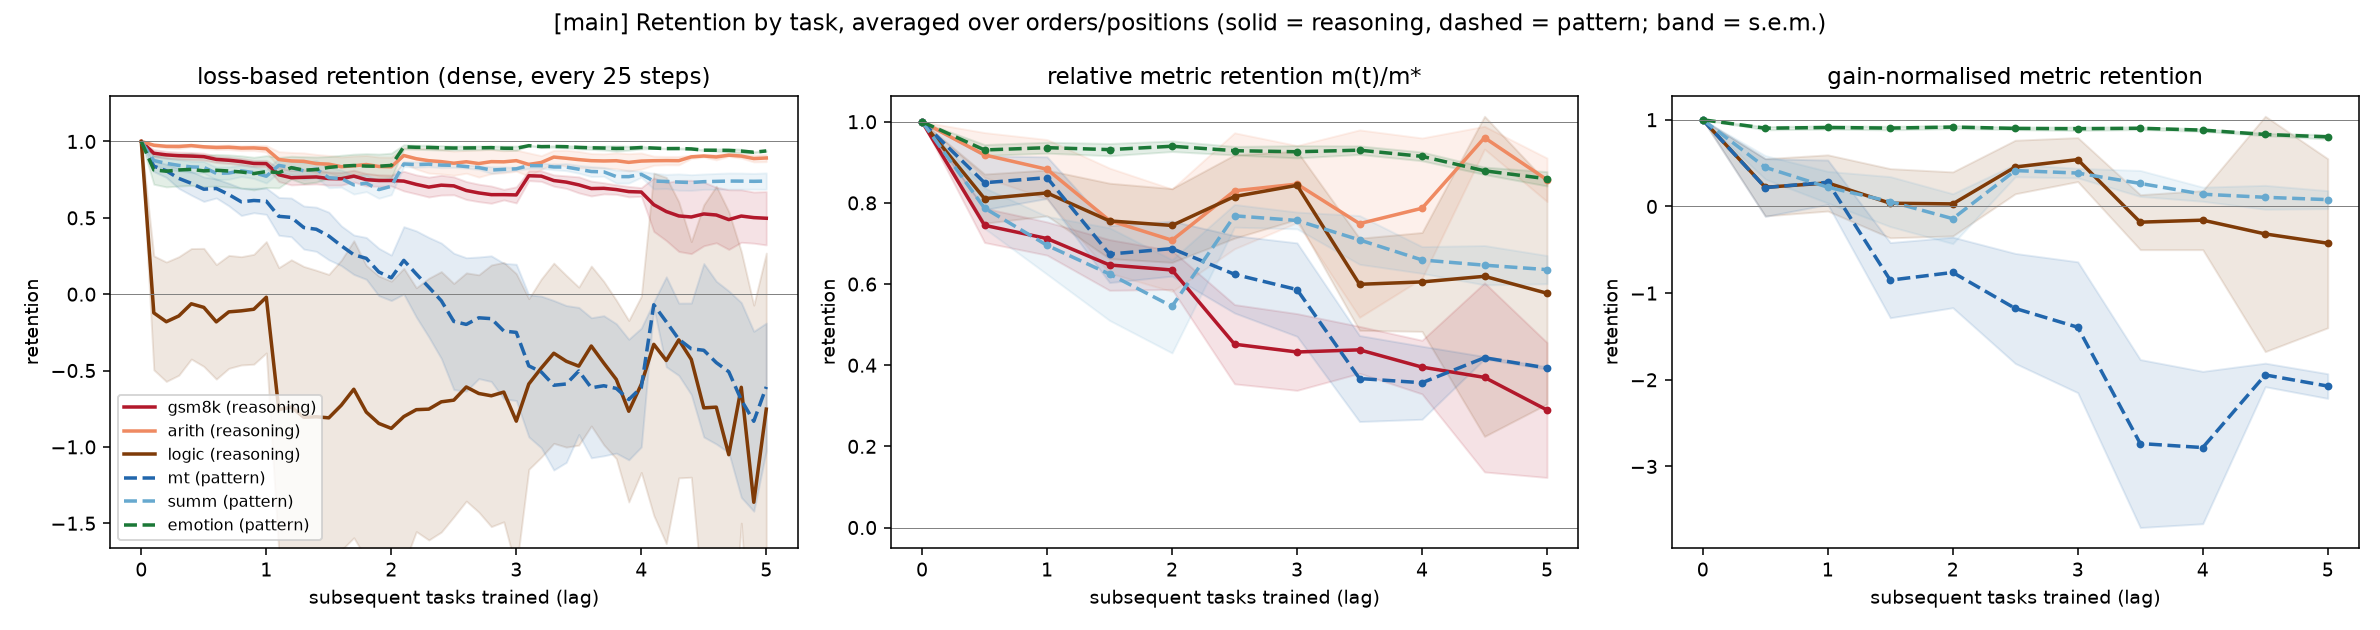
\includegraphics[width=\linewidth]{figures/main_retention_by_task.png}
    \caption{Retention by task on \llama, averaged over orders and positions (solid: reasoning; dashed: pattern; bands: s.e.m.). \figleft~Loss-based retention, every 25 steps. \figcenter~Relative metric retention. \figright~Gain-normalized retention (\tlogic, \tmt, \tsumm, \temo only). Several curves drop sharply right after a stage boundary (integer lags) and are flat, or even rising, for long stretches in between. \tlogic falls below zero-shot level in loss terms soon after the first switch.}
    \label{fig:retention}
\end{figure}

\begin{figure}[t]
    \centering
    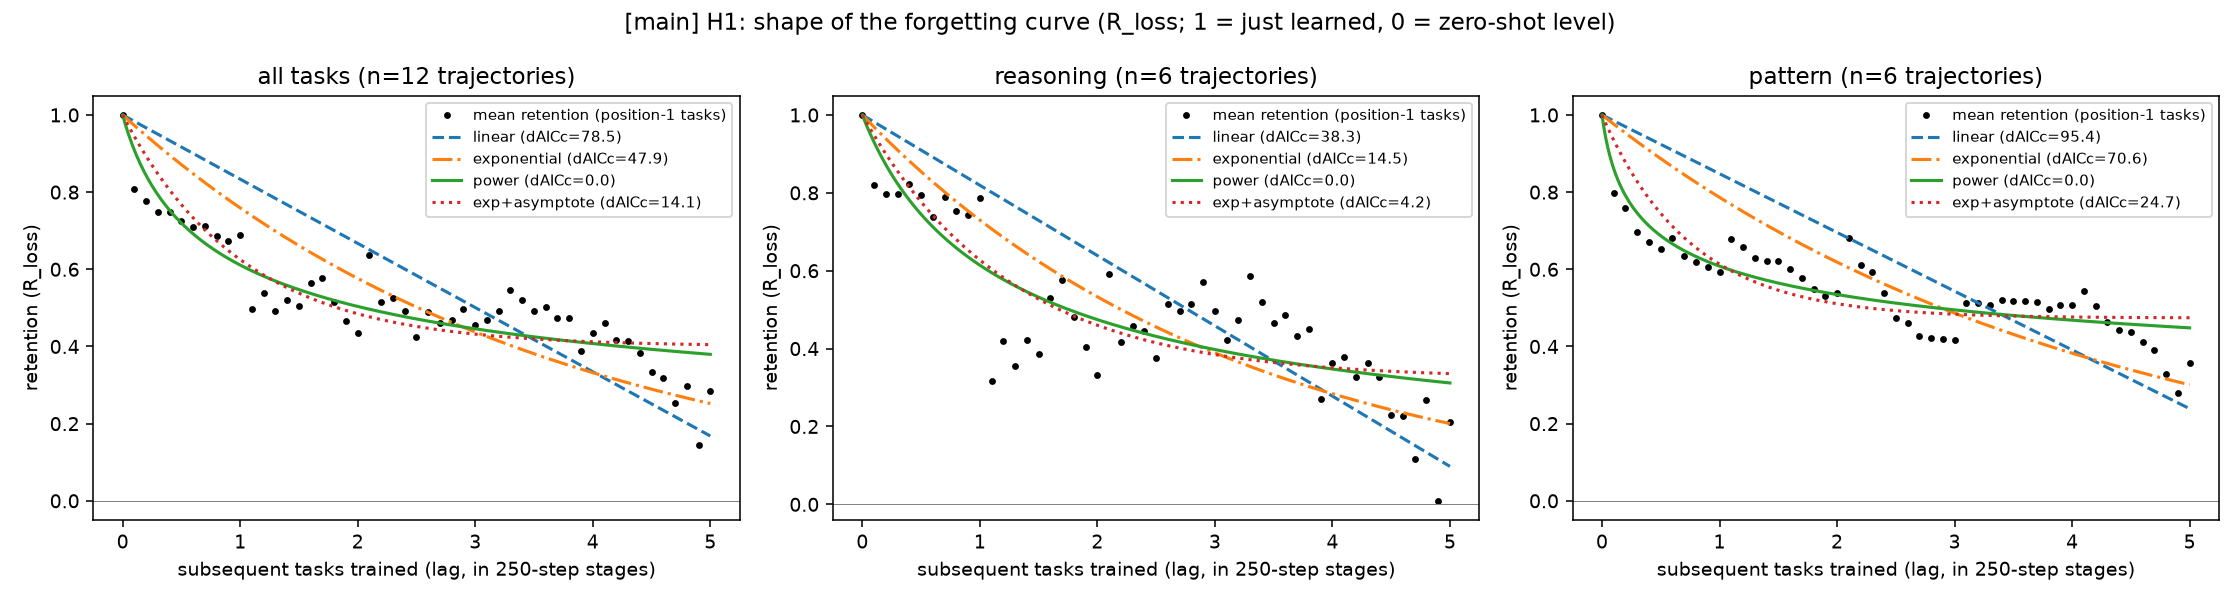
\includegraphics[width=\linewidth]{figures/main_h1_shape_R_loss.png}
    \caption{H1 fits to mean \rloss curves of position-1 tasks on \llama. The power law has the lowest AICc in all three panels, but the data points show steps at stage boundaries that no smooth monotone curve captures.}
    \label{fig:h1}
\end{figure}

\begin{table}[t]
    \centering
    \small
    \resizebox{\textwidth}{!}{%
    \begin{tabular}{@{}lccccc@{}}
        \toprule
        \textbf{Mean curve} & \textbf{Linear} & \textbf{Exponential} & \textbf{Power} & \textbf{Exp+asymptote} & \textbf{$R^2$ of best} \\
        \midrule
        \llama, all tasks, \rloss (12 traj.) & 78.5 & 47.9 & {\bf 0} & 14.1 & 0.81 \\
        \llama, reasoning, \rloss & 38.3 & 14.5 & {\bf 0} & 4.2 & 0.68 \\
        \llama, pattern, \rloss & 95.4 & 70.6 & {\bf 0} & 24.7 & 0.78 \\
        \llama, all tasks, \rrel (11 points) & 27.1 & 23.6 & {\bf 0} & 5.0 & 0.94 \\
        \midrule
        \qwen, all tasks, \rloss (6 traj.) & 82.5 & 28.9 & 8.7 & {\bf 0} & 0.35 \\
        \qwen, reasoning, \rloss & 54.7 & 46.8 & 6.6 & {\bf 0} & 0.08 \\
        \qwen, pattern, \rloss & 61.7 & {\bf 0} & 2.6 & 1.1 & 0.49 \\
        \bottomrule
    \end{tabular}
    }
    \caption{H1 on mean curves of position-1 tasks (pre-registered; lag axis in stages; 51 points per \rloss curve). Entries are \daicc relative to the best model ({\bf 0}); lower is better. The power law wins on the \llama averages and loses on the \qwen averages, where no smooth curve fits well.}
    \label{tab:h1_mean}
\end{table}

\begin{table}[t]
    \centering
    \small
    \begin{tabular}{@{}lcccc@{}}
        \toprule
        \textbf{Trajectories (positions 1--3)} & \textbf{Linear} & \textbf{Exponential} & \textbf{Power} & \textbf{Exp+asymptote} \\
        \midrule
        \llama, \rloss (36) & 9 & 4 & 2 & {\bf 21} \\
        \llama, \rrel (36) & 9 & {\bf 16} & 3 & 8 \\
        \qwen, \rloss (18) & 2 & 4 & 2 & {\bf 10} \\
        \qwen, \rrel (18) & 5 & {\bf 6} & 3 & 4 \\
        \bottomrule
    \end{tabular}
    \caption{H1 on individual trajectories: number of trajectories for which each model has the lowest AICc. Most frequent winner in {\bf bold}. The power law is the least frequent winner, or tied for it, in every row.}
    \label{tab:h1_traj}
\end{table}


{\bf Does the mean curve follow a power law?}
On \llama, yes; on \qwen, no.
\Tabref{tab:h1_mean} shows that linear decay is the worst model in every row, so uniform degradation is clearly rejected.
The power law wins all four \llama mean curves, with a margin of 4.2 to 24.7 AICc units over the saturating exponential.
On \qwen it wins none, and none of the four smooth curves fits well ($R^2 \leq 0.49$).
\Figref{fig:h1} shows the \llama fits.

{\bf Do individual trajectories follow a power law?}
No.
\Tabref{tab:h1_traj} shows that the power law has the lowest AICc in only 2 of 36 \llama trajectories and 2 of 18 \qwen trajectories under \rloss.
The power law and the exponential-to-asymptote both have two parameters, so we also compare just these two (exploratory).
On \llama the saturating exponential is clearly better ($\daicc > 2$) in 26 of 36 trajectories, the power law in 0, with 10 undecided; on \qwen the counts are 9, 2, and 7.
The per-task mean curves agree: the exponential-to-asymptote is best for 5 of 6 tasks on each model.
The power law therefore describes the average better than it describes the things being averaged.

{\bf Why do smooth curves fit poorly?}
Because forgetting comes in steps (\figref{fig:retention}).
We take all stage transitions in which an old task's loss rose by more than 0.02 nats over the stage (108 on \llama, 47 on \qwen).
On \llama the median share of the stage's rise that had already happened at the first evaluation, 25 of 250 steps in, is 55\%, and 72\% by step 50.
Uniform degradation predicts 10\% and 20\%.
On \qwen the shares are 39\% and 66\%.
The curves are also not monotone: in 21\% (\llama) and 24\% (\qwen) of all stage transitions an old task's loss went \emph{down} by more than 0.01 nats.
\Figref{fig:within} shows the mean loss increase within the first interfering stage.
On this within-stage mean the best fit is a power law with a very small exponent (0.07), which is itself close to a step; per trajectory, the saturating exponential wins most often (26 of 54, against 18 for the power law).
At 25-step resolution the two forms are hard to tell apart, which motivated the onset experiment.

\begin{figure}[t]
    \centering
    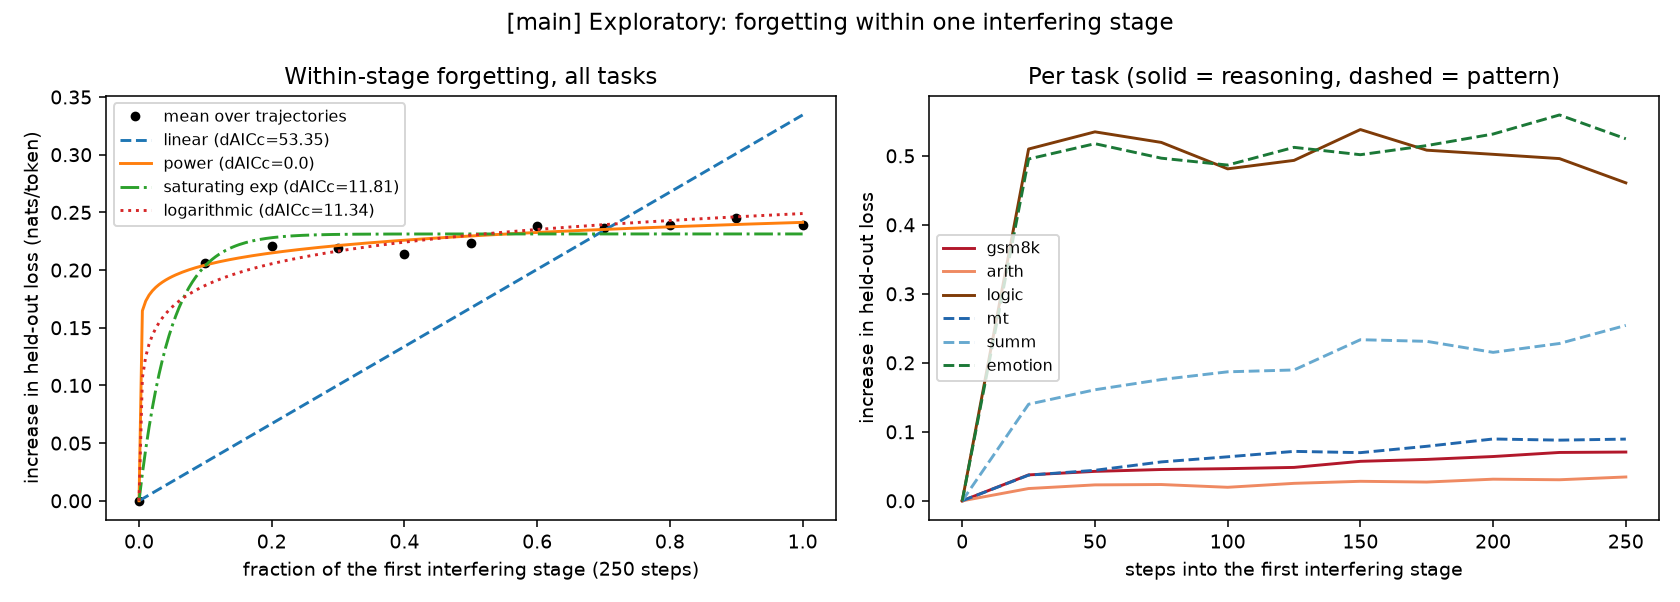
\includegraphics[width=0.95\linewidth]{figures/main_within_stage.png}
    \caption{Forgetting within the first interfering stage on \llama (exploratory). \figleft~Mean increase in old-task loss with four fits; almost all of the increase is present at the first evaluation point. \figright~The same by task. The step is large for \tlogic and \temo and small for \tgsm, \tarith, and \tmt.}
    \label{fig:within}
\end{figure}

\begin{figure}[t]
    \centering
    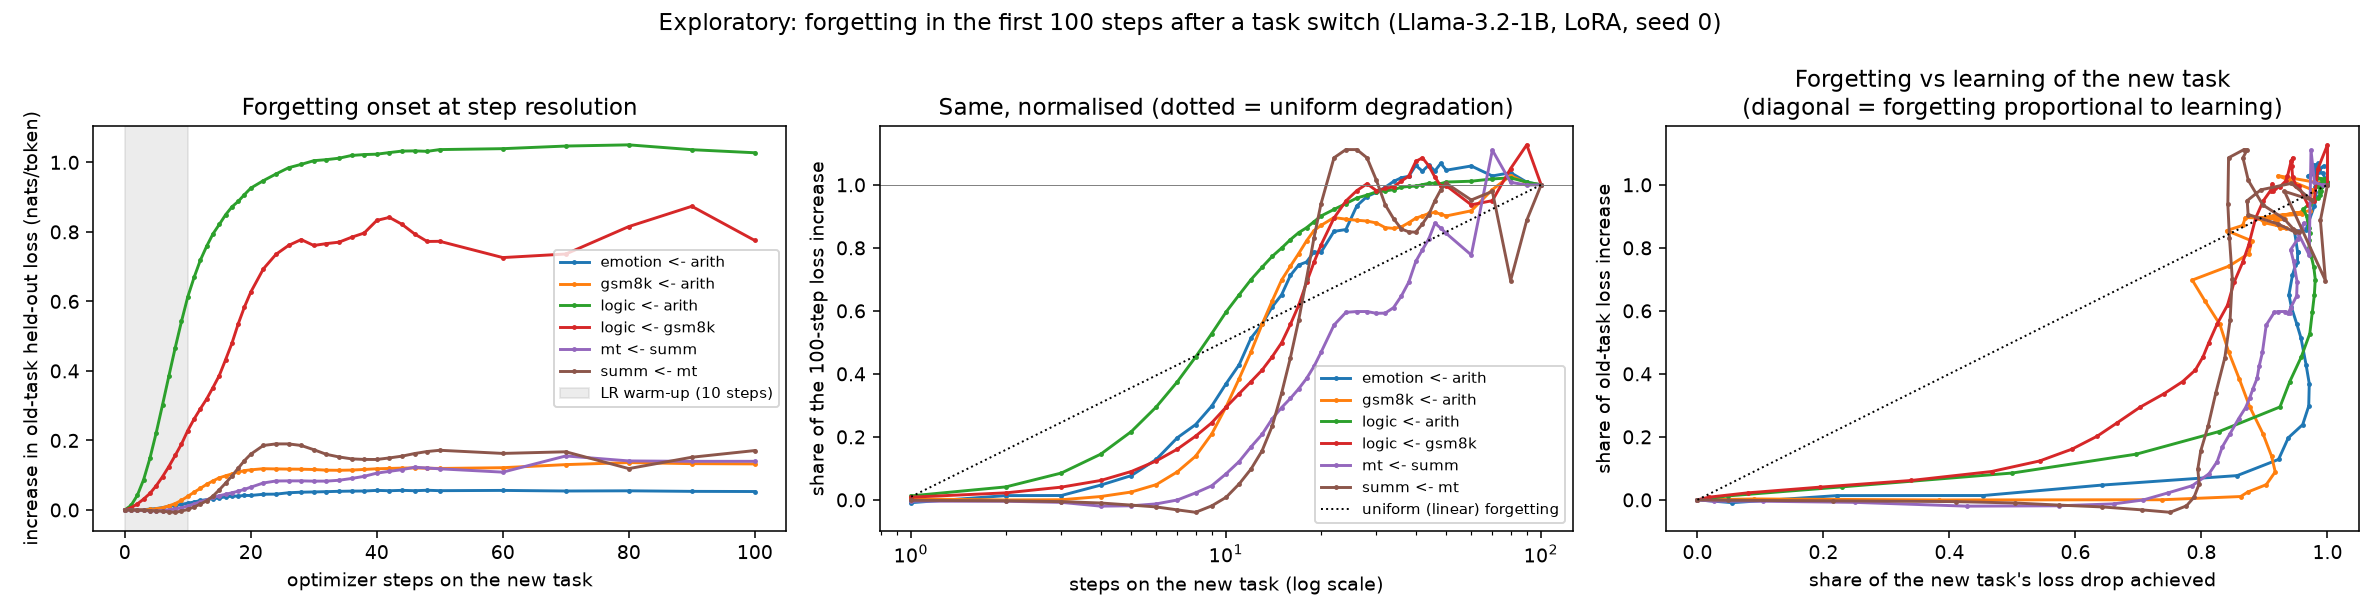
\includegraphics[width=\linewidth]{figures/onset.png}
    \caption{Onset of forgetting at step resolution (exploratory; \llama, six pairs, one seed). \figleft~Increase in old-task loss during the first 100 steps on a new task; the shaded region is the 10-step learning-rate warm-up. \figcenter~The same, normalized by the 100-step increase, on a log axis; the dotted line is uniform degradation. \figright~Forgetting of the old task against learning of the new task; forgetting lags behind learning.}
    \label{fig:onset}
\end{figure}

\begin{table}[t]
    \centering
    \resizebox{\textwidth}{!}{%
    \begin{tabular}{@{}lccccc@{}}
        \toprule
        & \textbf{Loss rise after} & \textbf{Share of rise reached} & \textbf{Old task: steps to} & \textbf{New task: steps to} & \textbf{\daicc, power vs.} \\
        \textbf{Old $\leftarrow$ new} & \textbf{100 steps (nats/token)} & \textbf{by step 10 / 20 / 50} & \textbf{50\% / 90\% of rise} & \textbf{50\% / 90\% of drop} & \textbf{saturating exp.} \\
        \midrule
        \tlogic $\leftarrow$ \tarith & 1.028 & 0.60 / 0.90 / 1.01 & 9 / 20 & 4 / 6 & $+74.9$ \\
        \tlogic $\leftarrow$ \tgsm & 0.775 & 0.29 / 0.81 / 1.00 & 16 / 24 & 6 / 26 & $+38.4$ \\
        \tsumm $\leftarrow$ \tmt & 0.171 & 0.01 / 0.94 / 1.00 & 17 / 20 & 4 / 34 & $+15.0$ \\
        \tmt $\leftarrow$ \tsumm & 0.140 & 0.08 / 0.47 / 0.85 & 22 / 70 & 5 / 22 & $+21.0$ \\
        \tgsm $\leftarrow$ \tarith & 0.132 & 0.30 / 0.87 / 0.90 & 13 / 42 & 3 / 6 & $+31.5$ \\
        \temo $\leftarrow$ \tarith & 0.053 & 0.37 / 0.79 / 1.05 & 12 / 26 & 4 / 6 & $+52.0$ \\
        \bottomrule
    \end{tabular}
    }
    \caption{Step-resolution onset of forgetting (exploratory; \llama, one seed). Positive \daicc means the saturating exponential fits better than the power law. Forgetting is mostly complete by step 20--50 and lags behind learning of the new task.}
    \label{tab:onset}
\end{table}


{\bf What does the onset look like at step resolution?}
\Figref{fig:onset} and \tabref{tab:onset} show the six pairs.
The saturating exponential is the best of the four candidates in all six pairs, and linear is the worst in all six (\daicc 32--149).
Between step 50 and step 100 the old-task loss changes by at most 0.022 nats.
The curves are slightly S-shaped: almost nothing happens in the first $\sim$5 steps, which coincides with the 10-step warm-up.
Forgetting also lags behind learning: the new task reaches half of its loss drop in 3--6 steps, the old task half of its loss rise in 9--22.
The warm-up is a property of our training recipe, so the delay may not generalize.

\para{Verdict on H1: not supported as stated.}
``Not uniform'' holds strongly.
``Power law'' holds only for averaged curves on one of two models.
The data are better described as a rapid, saturating step at each task switch whose size varies by task pair.
Summing such steps over a balanced set of interferers would give a decelerating average curve that a power law fits well; this reading is consistent with the fits above, but we did not test it directly.

\subsection{H2: No 3--5$\times$ Gap Between Reasoning and Pattern Tasks}
\label{sec:h2}

\begin{table}[t]
    \centering
    \resizebox{\textwidth}{!}{%
    \begin{tabular}{@{}lcccc@{}}
        \toprule
        & \multicolumn{2}{c}{\llama (12 runs)} & \multicolumn{2}{c}{\qwen (6 runs)} \\
        \cmidrule(lr){2-3} \cmidrule(lr){4-5}
        \textbf{Measure} & \textbf{Reas.\ / patt.} & \textbf{Ratio [95\% CI]} & \textbf{Reas.\ / patt.} & \textbf{Ratio [95\% CI]} \\
        \midrule
        \rloss (pre-registered) & 0.637 / 0.434 & 1.47 [1.05, 1.91] & 0.610 / 0.103 & 5.93 [$-12.9$, 32.5] \\
        \rrel (pre-registered) & 0.286 / 0.251 & 1.14 [0.82, 1.60] & 0.210 / 0.096 & 2.18 [1.08, 3.52] \\
        \rgain (pre-registered)$^\dagger$ & 0.843 / 0.954 & 0.88 [0.39, 1.56] & 0.505 / 0.399 & 1.27 [$-0.05$, 3.25] \\
        \absdrop & 0.165 / 0.124 & 1.33 [0.89, 1.90] & 0.157 / 0.060 & 2.60 [1.21, 4.21] \\
        \rloss clipped to $[0,1]$ (exploratory) & 0.349 / 0.347 & 1.01 [0.82, 1.26] & 0.453 / 0.374 & 1.21 [0.72, 1.95] \\
        \bottomrule
    \end{tabular}
    }
    \caption{H2: mean forgetting for reasoning and pattern tasks and their ratio, with cluster-bootstrap 95\% intervals over runs. Forgetting is $1 - R$ (or the absolute drop), averaged over all stage-end evaluations with lag $\geq 1$. H2 predicts a ratio in $[3, 5]$. $^\dagger$\tgsm and \tarith are excluded on both models and \tmt on \qwen, because fine-tuning gave no positive gain.}
    \label{tab:h2_ratio}
\end{table}

\begin{table}[t]
    \centering
    \small
    \begin{tabular}{@{}llcccccc@{}}
        \toprule
        & & \multicolumn{3}{c}{\llama} & \multicolumn{3}{c}{\qwen} \\
        \cmidrule(lr){3-5} \cmidrule(lr){6-8}
        \textbf{Task} & \textbf{Cat.} & \absdrop & $1-\rrel$ & $1-\rloss$ & \absdrop & $1-\rrel$ & $1-\rloss$ \\
        \midrule
        \tgsm & R & 0.153 & {\bf 0.435} & 0.264 & 0.104 & 0.231 & {\bf 0.954} \\
        \tarith & R & 0.168 & 0.186 & 0.109 & {\bf 0.282} & {\bf 0.288} & 0.562 \\
        \tlogic & R & {\bf 0.173} & 0.239 & {\bf 1.536} & 0.084 & 0.111 & 0.313 \\
        \tmt & P & 0.167 & 0.338 & 0.940 & 0.027 & 0.057 & $-0.044$ \\
        \tsumm & P & 0.139 & 0.341 & 0.236 & 0.034 & 0.100 & 0.215 \\
        \temo & P & 0.066 & 0.073 & 0.126 & 0.120 & 0.131 & 0.138 \\
        \bottomrule
    \end{tabular}
    \caption{Per-task forgetting (R = reasoning, P = pattern). Largest forgetting per column in {\bf bold}. Differences between tasks within a category are larger than the difference between categories, and the two models disagree on which tasks are fragile.}
    \label{tab:h2_pertask}
\end{table}


\Tabref{tab:h2_ratio} gives the category ratio under five measures, and \tabref{tab:h2_pertask} gives the per-task values behind it.

\para{\llama.}
No measure comes near 3.
The only interval that excludes 1 is unclipped \rloss (ratio 1.47; bootstrap one-sided $p = 0.016$, Holm-adjusted $p = 0.049$ over the three pre-registered measures).
One task carries this result: \tlogic spends 43\% of its cells \emph{below zero-shot level} in loss terms, and without \tlogic the ratio is 0.43.
Clipping gives 1.01.
The task-label permutation test gives $p = 0.7$.
In metric terms the three reasoning tasks and two of the three pattern tasks lose about the same (0.14--0.17); only \temo is robust.

\para{\qwen.}
The metric-based ratios are above 2, and their intervals exclude 1 (one-sided $p = 0.019$ for \rrel and $0.017$ for \absdrop) and overlap $[3, 5]$.
After Holm correction the \rrel result is $p = 0.057$.
The task-label permutation test gives $p = 0.2$--$0.3$; the smallest attainable value with six tasks is 0.1.
The unclipped loss ratio of 5.93 is not interpretable: \qwen barely improves on \tmt and \tgsm in loss terms ($L_0 - L^* = 0.033$ and $0.078$ nats), so the normalization divides by nearly zero, as the interval $[-12.9, 32.5]$ shows.
The largest metric drop on \qwen is \tarith (0.282) and the smallest are \tmt and \tsumm (about 0.03), but \qwen also gained almost nothing on \tmt from fine-tuning, so there was little to lose.

\para{Verdict on H2: not supported.}
A 3--5$\times$ gap is absent on \llama under every normalization.
\qwen shows a roughly 2.2--2.6$\times$ gap on metric-based measures that is suggestive but not robust to correction, to the choice of normalization, or to treating tasks instead of runs as the unit of generalization.
With three tasks per category, we cannot separate ``reasoning vs.\ pattern'' from ``these particular tasks''.

\subsection{H3: No Reliable Effect of Serial Position}
\label{sec:h3}

\begin{figure}[t]
    \centering
    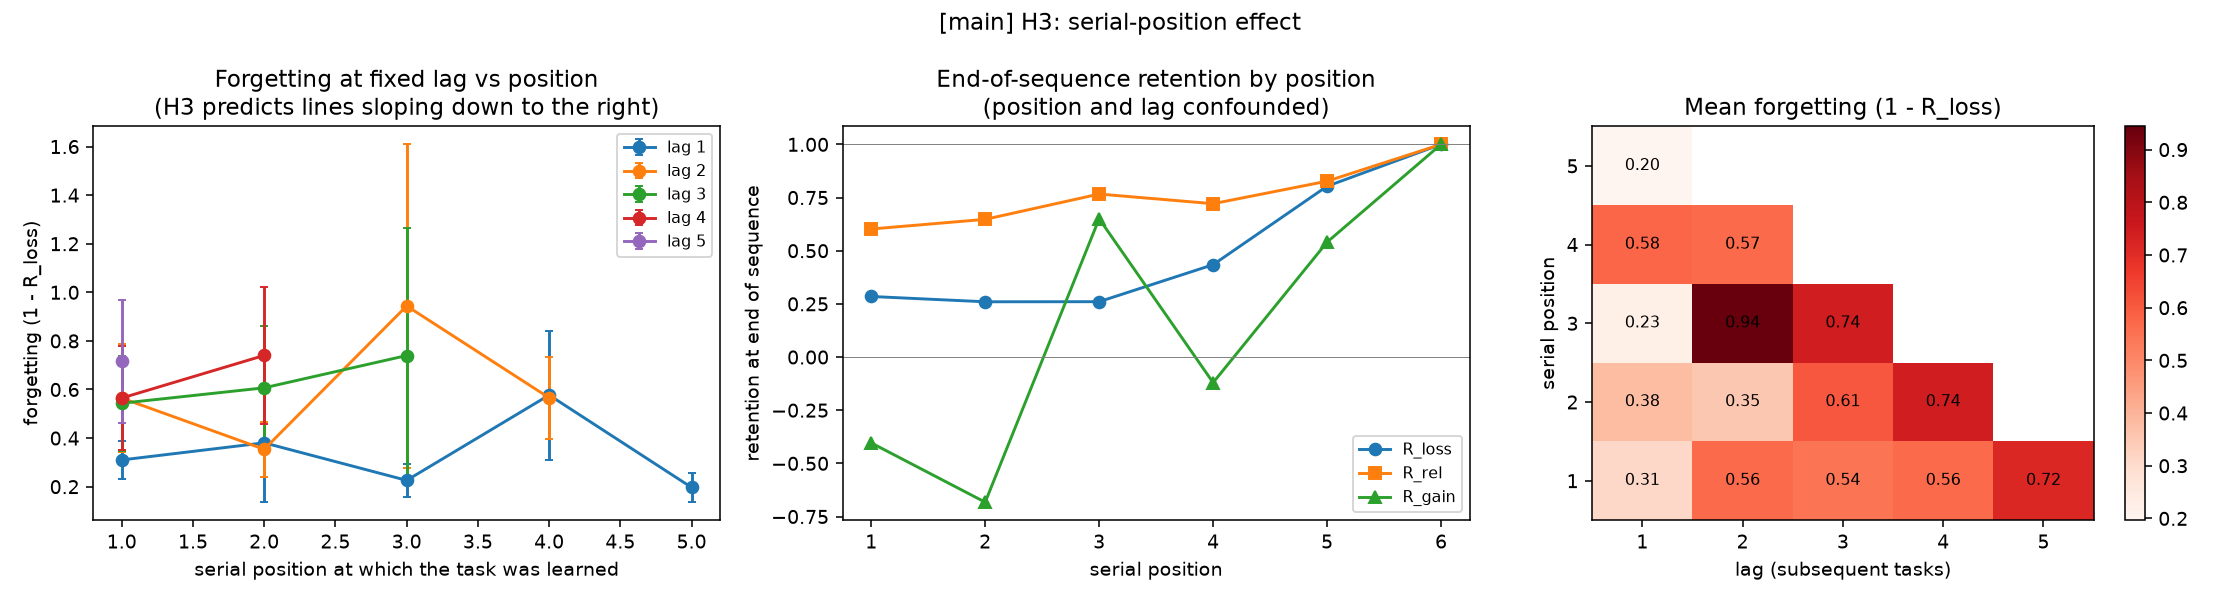
\includegraphics[width=\linewidth]{figures/main_h3_position.png}
    \caption{H3 on \llama, using unclipped \rloss. \figleft~Forgetting at fixed lag against serial position; H3 predicts lines sloping down to the right, which we do not see. \figcenter~End-of-sequence retention rises with position, but position and lag are confounded there. \figright~Mean forgetting by position and lag.}
    \label{fig:h3}
\end{figure}

\begin{table}[t]
    \centering
    \resizebox{\textwidth}{!}{%
    \begin{tabular}{@{}lcc@{}}
        \toprule
        & \llama (12 runs) & \qwen (6 runs) \\
        \midrule
        Lag-1 forgetting by position 1--5, \rloss clipped & 0.31, 0.21, 0.23, 0.38, 0.20 & 0.55, 0.51, 0.29, 0.23, 0.15 \\
        Spearman, position vs.\ lag-1 forgetting, \rloss clipped & $\rho = -0.06$, $p = 0.65$ & $\rho = -0.47$, $p = 0.009$ \\
        Same, \rrel & $\rho = 0.02$, $p = 0.87$ & $\rho = -0.18$, $p = 0.34$ \\
        Same, \rloss unclipped & $\rho = -0.12$, $p = 0.37$ & $\rho = -0.35$, $p = 0.055$ \\
        \midrule
        OLS position coefficient, \rloss clipped [95\% CI] & $-0.001$ [$-0.028$, 0.026] & $-0.073$ [$-0.138$, $-0.009$] \\
        OLS position coefficient, \rrel [95\% CI] & $-0.019$ [$-0.063$, 0.025] & $-0.019$ [$-0.047$, 0.009] \\
        OLS $\log(1+\text{lag})$ coefficient, \rrel [95\% CI] & 0.154 [0.015, 0.294] & $-0.039$ [$-0.206$, 0.128] \\
        \bottomrule
    \end{tabular}
    }
    \caption{H3: effect of serial position with lag held fixed. Spearman correlations use task-demeaned forgetting. A negative position coefficient is the direction H3 predicts (earlier-learned tasks forget more at the same lag). The $p$-values are uncorrected.}
    \label{tab:h3}
\end{table}


End-of-sequence retention does rise with position on both models; on \llama, \rrel is 0.60, 0.65, 0.77, 0.72, and 0.83 for positions 1--5 (\figref{fig:h3}, center).
But there, position and amount of subsequent training are the same thing.
\Tabref{tab:h3} holds lag fixed.

\llama shows no position effect on any measure: the Spearman correlations are between $-0.12$ and $0.02$, and both OLS position coefficients have intervals centered near zero.
\qwen shows the predicted direction on the clipped loss measure ($\rho = -0.47$, $p = 0.009$; OLS coefficient $-0.073$) and the same sign without significance on the metric measure.
These $p$-values are uncorrected across measures and models, and cluster-robust errors with six clusters are unreliable.

The two models also differ in how forgetting accumulates.
On \llama forgetting keeps growing with lag (log-lag coefficient 0.154 for \rrel).
On \qwen it does not measurably grow after the first subsequent task (coefficient $-0.039$, interval spanning zero).

\para{Verdict on H3: not supported on \llama; inconclusive on \qwen.}
On \llama the visible end-of-run disadvantage of early tasks is explained by their longer exposure to interference.

\subsection{What Does Predict Forgetting? Pair Structure and Output Format}
\label{sec:pairs}

\begin{table}[t]
    \centering
    \small
    \begin{tabular}{@{}lcccccc@{}}
        \toprule
        \textbf{Old $\backslash$ new} & \tgsm & \tarith & \tlogic & \tmt & \tsumm & \temo \\
        \midrule
        \tgsm & -- & 0.21 & 0.17 & 0.03 & 0.04 & 0.05 \\
        \tarith & 0.00 & -- & 0.16 & $-0.05$ & $-0.09$ & 0.14 \\
        \tlogic & {\bf 1.11} & {\bf 1.63} & -- & $-0.57$ & {\bf 0.91} & $-0.18$ \\
        \tmt & $-0.01$ & $-0.04$ & 0.14 & -- & {\bf 0.78} & {\bf 0.83} \\
        \tsumm & $-0.03$ & 0.02 & 0.13 & 0.17 & -- & 0.12 \\
        \temo & $-0.02$ & 0.19 & 0.04 & 0.02 & 0.02 & -- \\
        \bottomrule
    \end{tabular}
    \caption{Pair structure on \llama: mean loss-based retention (\rloss) lost by an old task (row) during one stage of training on a new task (column). Negative values are recovery. The five largest cells are in {\bf bold}; they carry most of the forgetting.}
    \label{tab:interference}
\end{table}

\begin{table}[t]
    \centering
    \small
    \begin{tabular}{@{}lccc@{}}
        \toprule
        & \multicolumn{2}{c}{\llama} & \qwen \\
        \cmidrule(lr){2-3} \cmidrule(lr){4-4}
        \textbf{Task} & \textbf{Format valid} & \textbf{Score given valid format} & \textbf{Format valid} \\
        \midrule
        \tgsm & 0.99 $\rightarrow$ 0.70 & 0.35 $\rightarrow$ 0.21 & 1.00 $\rightarrow$ 0.75 \\
        \tarith & 1.00 $\rightarrow$ 0.73 & 0.93 $\rightarrow$ 0.79 & 1.00 $\rightarrow$ 0.68 \\
        \tlogic & 1.00 $\rightarrow$ 0.73 & 0.68 $\rightarrow$ 0.61 & 1.00 $\rightarrow$ 0.96 \\
        \tmt & 0.99 $\rightarrow$ 0.62 & 0.49 $\rightarrow$ 0.36 & 1.00 $\rightarrow$ 0.99 \\
        \tsumm & 1.00 $\rightarrow$ 0.75 & 0.40 $\rightarrow$ 0.28 & 1.00 $\rightarrow$ 0.96 \\
        \temo & 1.00 $\rightarrow$ 0.87 & 0.90 $\rightarrow$ 0.84 & 1.00 $\rightarrow$ 0.99 \\
        \bottomrule
    \end{tabular}
    \caption{Format versus content. Each entry is (just learned $\rightarrow$ after later tasks). ``Format valid'' is the share of outputs with the requested form (\eg contains \texttt{Answer:}, is one of the allowed labels, is not an echo of the source). On \llama both the output format and the score among well-formatted outputs erode.}
    \label{tab:format}
\end{table}


\para{Pair structure.}
\Tabref{tab:interference} shows how much retention each old task loses during one stage of each new task on \llama.
A handful of pairs carry most of the forgetting: \tlogic after \tarith, \tgsm, or \tsumm, and \tmt after \tsumm or \temo.
Some pairs produce recovery, such as \tlogic after \tmt ($-0.57$).
On \llama, same-category pairs average 0.435 against 0.039 for cross-category pairs.
This contrast rests on those few cells and does not replicate on \qwen ($-0.219$ vs.\ 0.023), where the \tmt row is distorted by the near-zero loss denominator.
On \qwen, \tlogic is the most damaging \emph{interferer} and not the most damaged task (\tabref{tab:qwen_interference}).

\para{Format versus content.}
We check each stored generation for the requested output form (\tabref{tab:format}).
On \llama every task loses its output format in 13--38\% of later outputs, and the score also falls among outputs that keep the format.
Both the interface and the content erode.
On \qwen, format loss is confined to \tgsm and \tarith, the two tasks with multi-line worked answers.
Typical failures after a later task has been trained are an arithmetic answer written as prose without the \texttt{Answer:} line after summarization training, and a GSM8K problem that is paraphrased instead of solved.

\section{Discussion}
\label{sec:discussion}

\para{Forgetting is event-driven.}
The hypothesis pictured forgetting as a smooth process in training time with a task-type-specific rate.
The trajectories show something else: a switch of training distribution causes a fast, bounded shift, after which continued training on the same new task does little further harm.
A ``rate per step'' is then not a natural quantity; ``loss per switch, by pair'' is.
For practice, this means that evaluating shortly after a switch already shows most of the damage, and that training longer on the new task adds little further loss in our setting.

\para{Why does a power law appear in averages?}
The \llama average is well fit by a power law with a small exponent, and so would be many decelerating curves.
The equal-parameter comparison on individual trajectories and the step-resolution experiment both favor saturation.
This matches the known result that averaging can produce power-like curves from components that are not power laws~\cite{anderson1997artifactual}.
We did not run a simulation showing that the observed mixture of steps reproduces the averaged power-law fit, so this remains the most economical reading and not a demonstrated mechanism.

\para{The two models disagree.}
\llama and \qwen disagree on which tasks are fragile (\llama: \tlogic and \tmt; \qwen: \tarith and \tgsm), on whether forgetting accumulates with lag, and on the category ratio.
Any claim of a universal reasoning-vs.-pattern constant would need many more tasks and models than we have.

\para{Normalization matters.}
The same \llama data give a category ratio from 0.88 to 1.47 depending on the measure, and the same \qwen data from 1.2 to 5.9.
Loss-normalized retention breaks down when fine-tuning barely changes a task's loss.
Cross-task forgetting numbers quoted without their normalization are not comparable.

\subsection{Limitations}
\label{sec:limitations}

\para{Scale and method.}
We study 1B and 1.5B models with LoRA at $r{=}16$, one learning rate, 250 steps per task, and no replay or regularization.
We planned a full-fine-tuning ablation and cancelled it before any of its runs started because of GPU contention and time, so nothing here speaks to full fine-tuning or to larger models.

\para{Tasks.}
We use six tasks, three per category, with a debatable category assignment.
Tasks are the real unit of generalization for H2, and there are too few for a powerful test.
Fine-tuning hurt \tgsm accuracy and did not improve \tarith (both models) or \tmt (\qwen).
Forgetting of something that was barely learned is hard to define, and the gain-normalized results rest on 3--4 tasks.

\para{Statistical power.}
Each test set has 200 items, so single accuracy differences below about 7 points are within sampling error; our conclusions rest on aggregates over runs.
The two \llama blocks differ in both seed and order set, so we cannot separate the two.
\qwen has one block and one joint-baseline seed.

\para{Onset experiment.}
It uses one seed, six pairs chosen partly because they showed strong interference in the main runs, \llama only, and losses only.
The S-shaped start coincides with the learning-rate warm-up, and we did not test it without warm-up.

\para{Curve fitting.}
All four pre-registered models are monotone and start at 1, while real trajectories are non-monotone in over 20\% of transitions.
AICc treats the 51 points of a mean curve as independent, which they are not, so the \daicc magnitudes overstate certainty; the win counts are the safer evidence.

\para{Exploratory analyses.}
We added the clipped loss measure, the within-stage fits, the equal-parameter comparison, the sensitivity checks, and the onset experiment after seeing the main results.
The format-validity checks are simple string rules that we validated only by spot checks.

\para{Reproducibility.}
Runs are seeded, but our out-of-memory handling changes micro-batch sizes, so floating-point summation order can differ between repeats.
We do not expect bit-level reproduction and did not repeat a training run to measure the variation.
The analysis scripts are deterministic.

\para{Literature.}
We did not run a systematic literature search for this study.
Our positioning against prior work in \secref{sec:related} reflects our general knowledge of the cited papers, which we did not re-read for this study.

\section{Conclusion}
\label{sec:conclusion}

We tested whether forgetting in continual instruction tuning follows a power law, hits reasoning tasks 3--5$\times$ harder than pattern-matching tasks, and hits early-learned tasks disproportionately.
In naive sequential LoRA tuning of two small LLMs, none of the three holds as stated.
Forgetting is neither uniform nor well described as a per-task power law: it arrives as a fast, saturating hit at each task switch.
Reasoning tasks are not forgotten 3--5$\times$ faster (about 1$\times$ on \llama, about 2$\times$ with wide uncertainty on \qwen), and early-learned tasks are not forgotten disproportionately on \llama once exposure is controlled.
Which specific task follows which is the strongest visible determinant.

The key takeaway is that, in this setting, the forgetting tax is charged per task switch, almost immediately, and its size depends on the pair.

Several follow-ups would sharpen this picture.
First, we would repeat the onset experiment without warm-up, at several learning rates, with more seeds, and on \qwen, to see whether the saturation time scales with learning rate as a step-size effect would.
Second, we would test whether the per-switch hit is predictable from gradient or representation overlap between the two tasks, as the pair matrix suggests.
Third, we would run 15--20 tasks per category so that category can be tested with tasks as the unit, reinstate the full-fine-tuning ablation, and add a larger model.
Finally, we would simulate averaged curves from fitted per-switch steps to check directly whether aggregation alone reproduces the power-law fit.


\bibliography{references}

\appendix
\section{Additional Results for \qwen}
\label{app:qwen}

\Tabref{tab:qwen_baselines} gives the per-task baselines for \qwen, and \tabref{tab:qwen_interference} the pair matrix.
\Figref{fig:qwen_retention}, \figref{fig:qwen_h1}, and \figref{fig:qwen_h3} repeat the main figures for \qwen.

\begin{table}[h]
    \centering
    \small
    \begin{tabular}{@{}lcccc@{}}
        \toprule
        \textbf{Task} & \textbf{Zero-shot} & \textbf{End of own stage} & \textbf{Sequential, end of run} & \textbf{Joint multi-task} \\
        \midrule
        \tgsm & {\bf 0.475} & 0.461 & 0.376 {\scriptsize (0.153)} & 0.430 \\
        \tarith & {\bf 0.985} & 0.981 & 0.839 {\scriptsize (0.195)} & 0.975 \\
        \tlogic & 0.595 & {\bf 0.712} & 0.622 {\scriptsize (0.108)} & 0.680 \\
        \tmt & {\bf 0.469} & 0.465 & 0.436 {\scriptsize (0.035)} & 0.466 \\
        \tsumm & 0.269 & {\bf 0.338} & 0.309 {\scriptsize (0.012)} & 0.324 \\
        \temo & 0.500 & {\bf 0.910} & 0.817 {\scriptsize (0.108)} & 0.855 \\
        \midrule
        Mean & 0.549 & {\bf 0.644} & 0.567 & 0.622 \\
        \bottomrule
    \end{tabular}
    \caption{Per-task metrics on \qwen (6 sequential runs; joint training 1 seed; standard deviation over runs in parentheses). Best value per row in {\bf bold}. Fine-tuning does not improve \tgsm, \tarith, or \tmt.}
    \label{tab:qwen_baselines}
\end{table}

\begin{table}[h]
    \centering
    \small
    \begin{tabular}{@{}lcccccc@{}}
        \toprule
        \textbf{Old $\backslash$ new} & \tgsm & \tarith & \tlogic & \tmt & \tsumm & \temo \\
        \midrule
        \tgsm & -- & 0.34 & 1.07 & 0.09 & $-0.06$ & $-0.12$ \\
        \tarith & $-0.70$ & -- & 1.46 & 0.01 & $-0.93$ & 0.53 \\
        \tlogic & $-0.07$ & 0.33 & -- & $-0.07$ & 0.10 & 0.19 \\
        \tmt & $-0.11$ & $-0.58$ & 1.13 & -- & $-3.56$ & $-1.78$ \\
        \tsumm & $-0.08$ & $-0.10$ & 0.30 & 0.06 & -- & 0.11 \\
        \temo & 0.02 & 0.05 & 0.06 & 0.03 & 0.06 & -- \\
        \bottomrule
    \end{tabular}
    \caption{Pair structure on \qwen: mean \rloss lost by an old task (row) during one stage of a new task (column). The \tlogic column is the largest in four of the five rows. The \tmt row is distorted by a near-zero denominator ($L_0 - L^* = 0.033$ nats).}
    \label{tab:qwen_interference}
\end{table}

\begin{figure}[h]
    \centering
    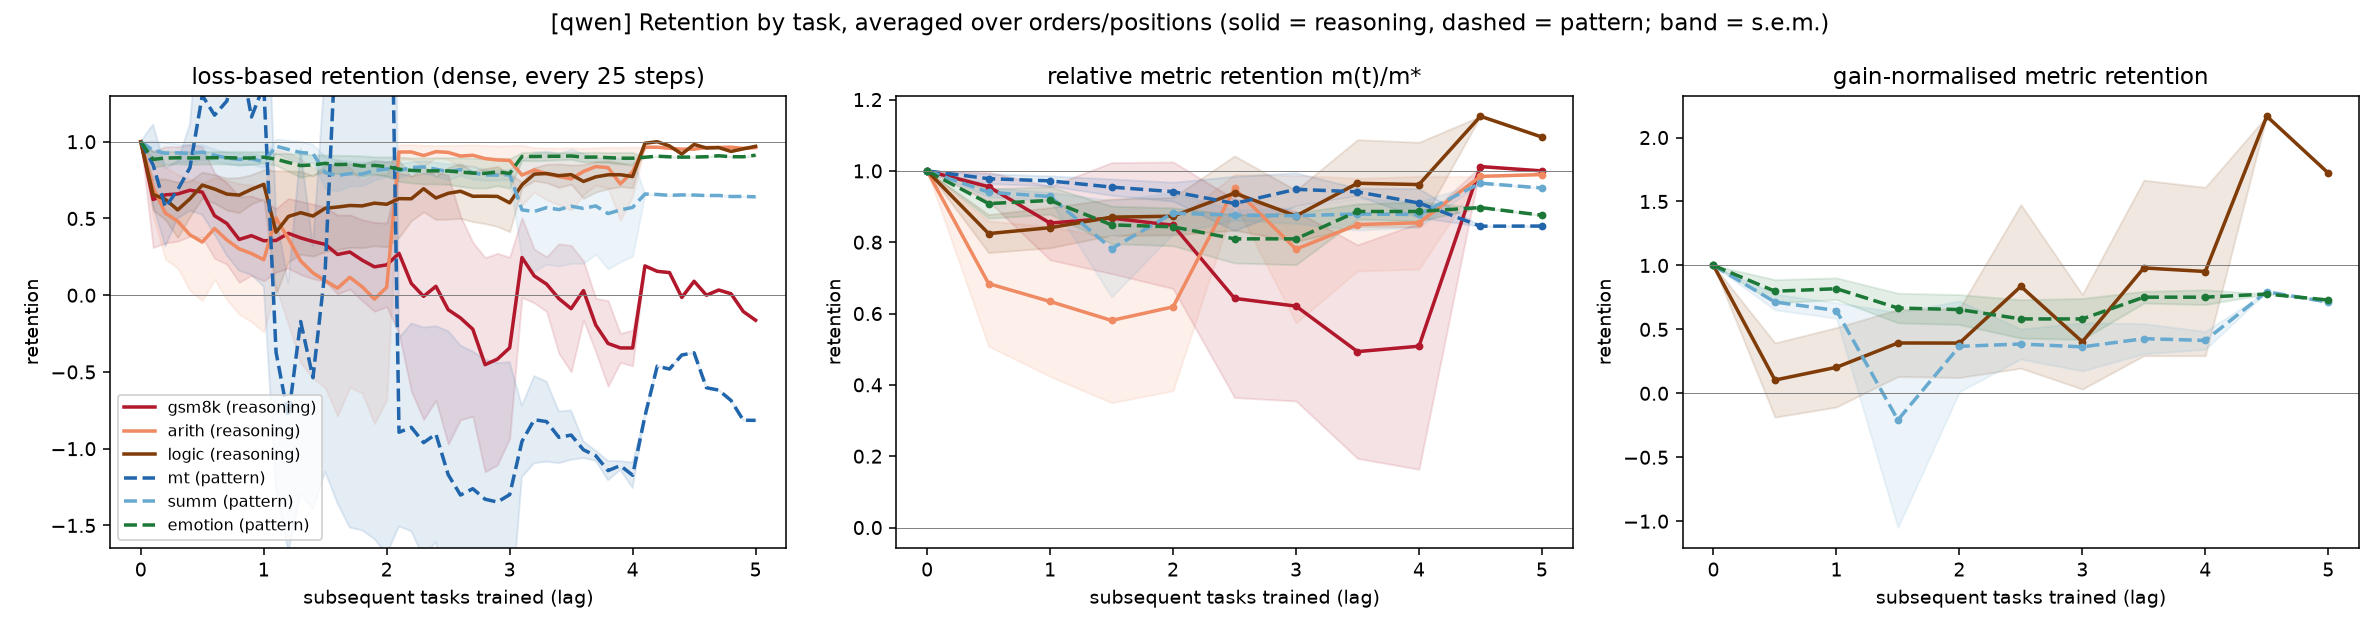
\includegraphics[width=\linewidth]{figures/qwen_retention_by_task.png}
    \caption{Retention by task on \qwen, averaged over orders and positions. Panels as in \figref{fig:retention}.}
    \label{fig:qwen_retention}
\end{figure}

\begin{figure}[h]
    \centering
    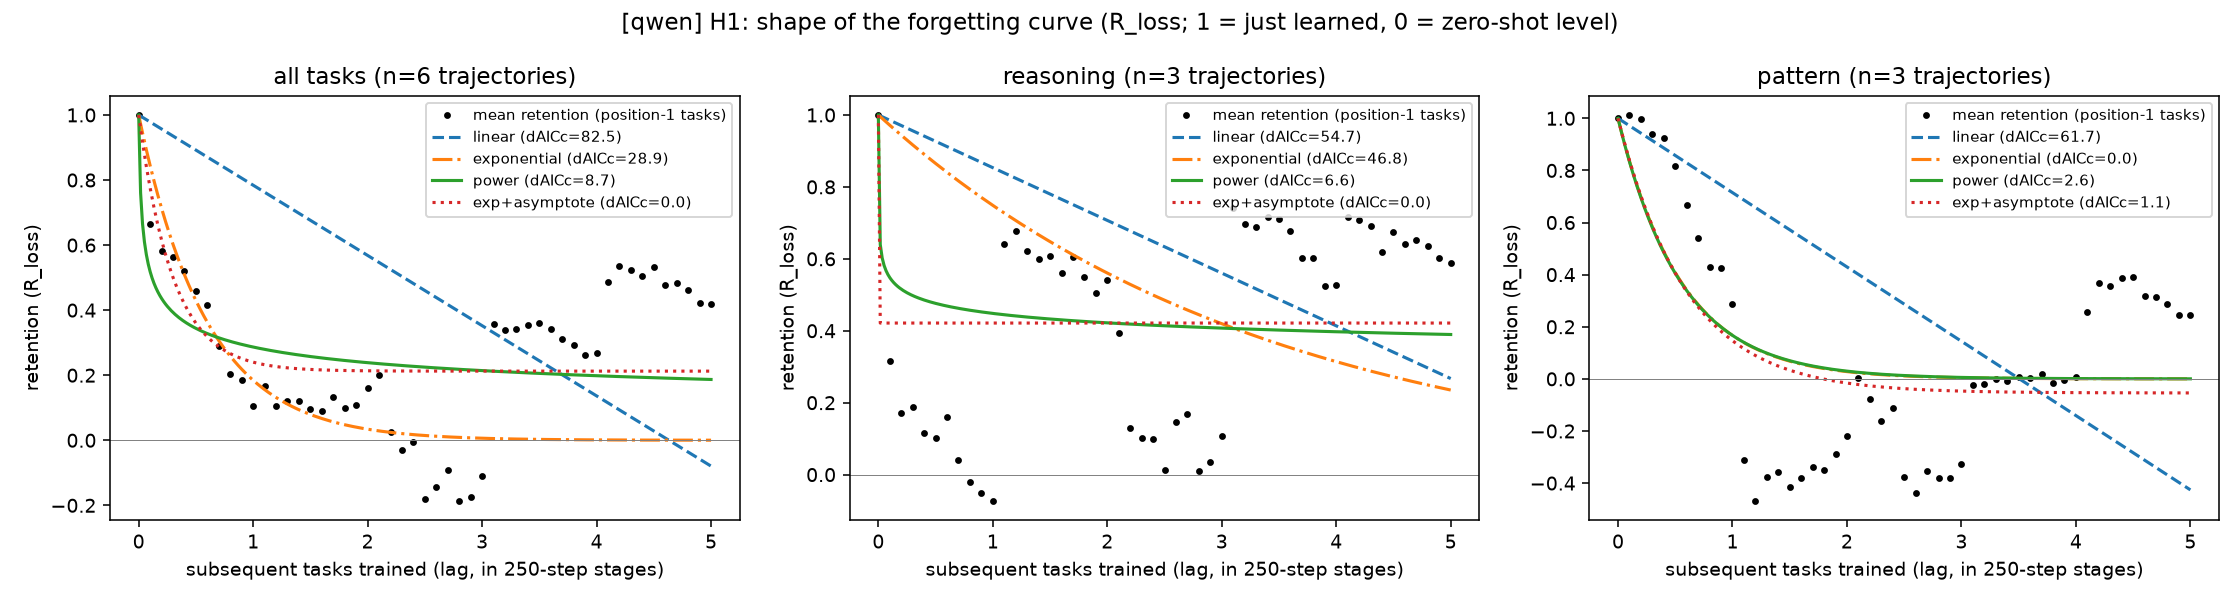
\includegraphics[width=\linewidth]{figures/qwen_h1_shape_R_loss.png}
    \caption{H1 fits to mean \rloss curves of position-1 tasks on \qwen. No smooth curve fits well (\tabref{tab:h1_mean}).}
    \label{fig:qwen_h1}
\end{figure}

\begin{figure}[h]
    \centering
    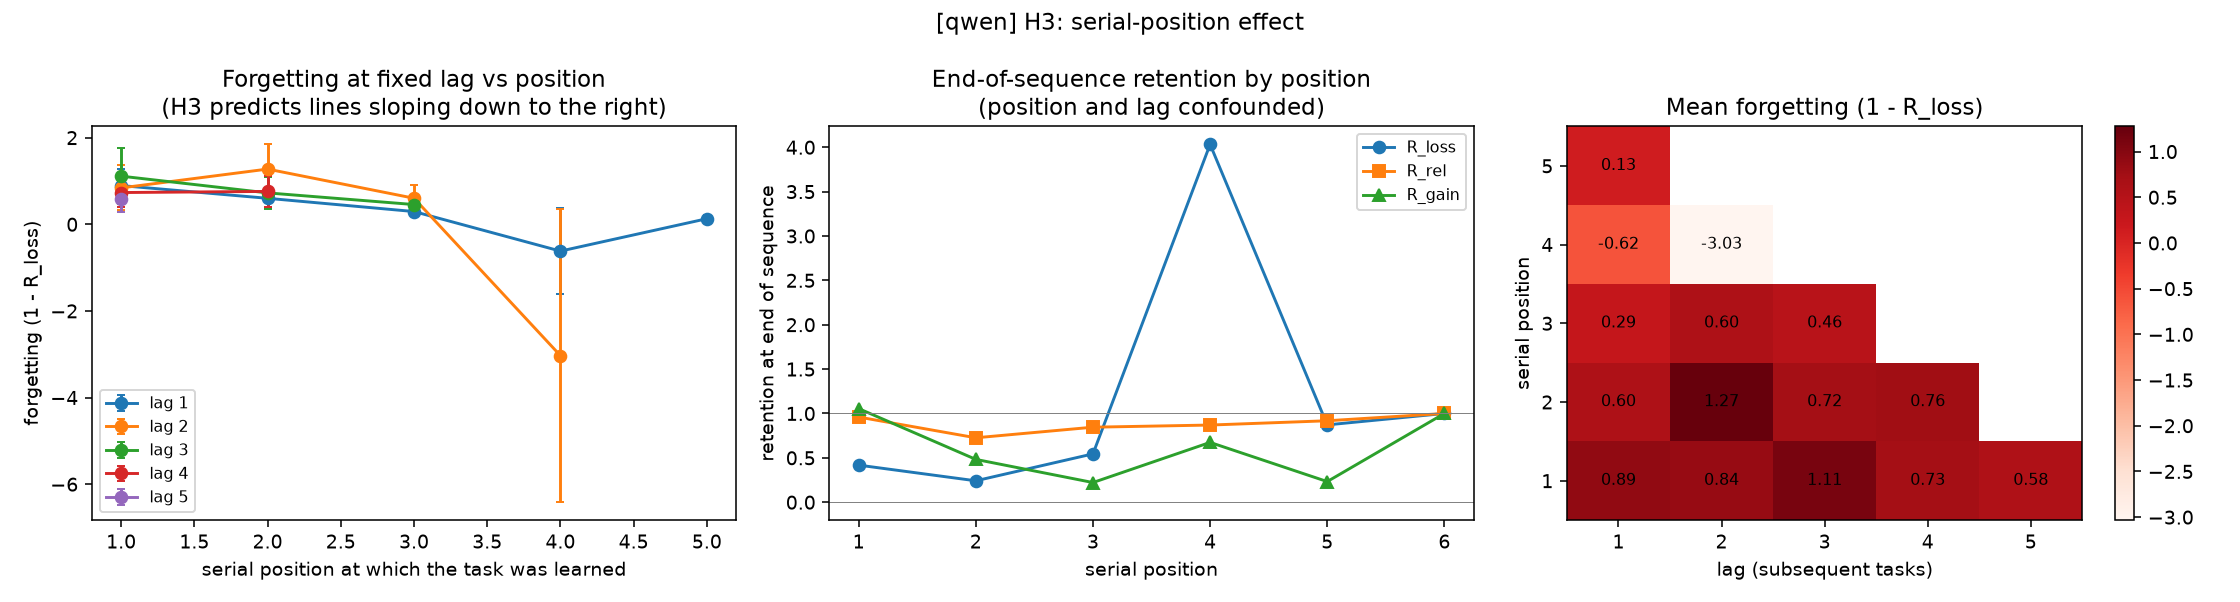
\includegraphics[width=\linewidth]{figures/qwen_h3_position.png}
    \caption{H3 on \qwen. Panels as in \figref{fig:h3}.}
    \label{fig:qwen_h3}
\end{figure}

\section{Sensitivity of the H2 Ratio on \llama}
\label{app:sensitivity}

We ran two exploratory sensitivity checks on the \llama category ratio.
By seed block, the unclipped \rloss ratio is 1.82 in block 0 and 1.15 in block 1; the clipped ratio is 1.06 and 0.95; the \rrel ratio is 1.23 and 1.07; and the \absdrop ratio is 1.43 and 1.24.
Leaving one task out, the unclipped \rloss ratio is 1.90 without \tgsm, 2.07 without \tarith, 0.43 without \tlogic, 3.52 without \tmt, 1.19 without \tsumm, and 1.08 without \temo.
The ratio therefore depends strongly on which single task is in or out of the comparison.

\section{Deviations from the Pre-registered Plan}
\label{app:deviations}

We wrote the analysis plan before any training run.
We deviated from it as follows.
\begin{itemize}[leftmargin=*,itemsep=0pt,topsep=0pt]
    \item \textbf{Evaluation cadence} (before any run). We planned loss and generation every 50 steps. We changed this to loss every 25 steps and generation every 125 steps, because generation costs about 45 seconds per evaluation point and loss about 3 seconds.
    \item \textbf{Generation budgets} (before any run). We raised the budgets for \tgsm and \tarith to 320 and 160 tokens, because a smoke test showed that verbose zero-shot answers were truncated before the final answer, which would have understated the zero-shot floor.
    \item \textbf{Full-fine-tuning ablation.} We cancelled it before any of its runs started. The GPUs were shared with other jobs, LoRA runs took up to about 100 minutes instead of about 10, and full fine-tuning needs about three times the memory. No full-fine-tuning data exists.
    \item \textbf{Restarts.} Two main runs and the \qwen joint baseline died with out-of-memory errors and were restarted from scratch with the same seed and configuration. We use no partial runs in any analysis.
    \item \textbf{Exploratory additions} (after seeing the main results). The clipped \rloss measure, the within-stage shape analysis, the equal-parameter per-trajectory comparison, the seed-block and leave-one-task-out sensitivity checks, and the onset experiment. A first attempt to get step resolution by re-running two full sequences with evaluation every 5 steps was aborted after 10 minutes because of its projected cost; we use no results from it.
\end{itemize}

\section{Compute and Software}
\label{app:compute}

We ran 18 sequential runs (12 on \llama, 6 on \qwen), 3 joint-training runs (2 on \llama, 1 on \qwen), and the six short onset runs on four shared NVIDIA RTX A6000 GPUs (48 GB), with a peak of 28 GB per process and bf16 autocast.
The full runs took 29.5 GPU-process-hours in total; because the GPUs were shared, single runs took 60--110 minutes.
We used no API models.
Software: Python 3.14.2, PyTorch 2.14.1, transformers 5.19.0, peft 0.21.2, SciPy 1.18.1, statsmodels 0.15.0, NumPy 2.5.3, and pandas 3.0.6.


\end{document}
